% CSE Seminararbeit
% Thema: Ein auf Neuronalen Netzen basierendes Ensemble-Modell zur Windprognose
% Autoren: Alicia Pirwass, Daniel Müller

\documentclass[
12pt, %Schriftgröße
toc=listofnumbered, %Tab.- & Abb.verzeichnis ins TOC
toc=chapterentrydotfill, %TOC: Punkte auch nach Kapitel
numbers=noenddot, %Kapitelüberschrift: Kein Endpunkt z.B. 2.2. --> 2.2
captions=tableheading, %Mehr Platz bei Captionüberschriften (Tabelle)
bibliography=numbered
]{scrreprt}


%%%%% SCHRIFTSATZ, SPRACHE, SCHRIFTART
%%% USE WITH pdflatex, siehe https://tex.stackexchange.com/a/44701
%\usepackage[T1]{fontenc}
%\usepackage[utf8]{inputenc}
%%% USE WITH xelatex
\usepackage{fontspec}
\defaultfontfeatures{Ligatures=TeX}
%%% USE WITH lualatex
%\usepackage{luatextra}
%\defaultfontfeatures{Ligatures=TeX}
%%%
\usepackage[ngerman]{babel}
% Nur mit LuaTex Interpreter nutzbar
%\usepackage{mathfont} % Dieses Packet läd auch fontspec
%\setmainfont{Segoe Pro} % Textschrift separat setzen


%%%%% INHALTSVERZEICHNIS
%\setuptoc{toc}{numbered} % TOC ins TOC, benötigen wir hier nicht 
%\addtokomafont{chapterentrypagenumber}{\normalfont\textbf}

\addtokomafont{disposition}{\rmfamily}
\addtokomafont{chapterentry}{\textbf}
\RedeclareSectionCommand[tocnumwidth=2.5em]{chapter}
\RedeclareSectionCommand[tocnumwidth=2.5em,tocindent=2.5em]{section}
\RedeclareSectionCommand[tocnumwidth=2.5em,tocindent=5em]{subsection}
%\newcounter{romanchapter} Benötigen wir nur, wenn z.B. Abstract, Literaturverz. und Anhang römisch nummeriert werden soll


%%%%% MATHEMATIK
\usepackage{amssymb, amsmath}
\usepackage{isomath}
\usepackage{pifont} % Für \cmark und \xmark
\newcommand{\cmark}{\ding{51}}%
\newcommand{\xmark}{\ding{55}}%


%%%%% BIBLIOGRAPHIE
\usepackage[style=ieee, mincitenames=1, maxcitenames=1]{biblatex}
\usepackage{url} % Damit URLs in der Quelle schön umgebrochen werden
\setcounter{biburllcpenalty}{7000} % Einstellungen für Packet url
\setcounter{biburlucpenalty}{8000} % Einstellungen für Packet url
\DefineBibliographyStrings{ngerman}{andothers = {{et\,al\adddot}},}
\addbibresource{bib.bib} %
\usepackage{csquotes}
%\emergencystretch=1em
\usepackage[final]{microtype}
%\usepackage[expansion, final]{microtype}
%\usepackage{natbib}
%\setcounter{biburlnumpenalty}{9000}
%\setcounter{biburllcpenalty}{9000}
%\setcounter{biburlucpenalty}{9000}


%%%%% ANHANG
\usepackage{appendix}


%%%%% FARBEN
\usepackage[table,xcdraw]{xcolor}
\definecolor{color20}{RGB}{35,35,35}
\definecolor{color25}{RGB}{69,69,69}
\definecolor{color30}{RGB}{80,80,80}
\definecolor{color80}{RGB}{190,190,190}


%%%%% ÜBERSCHRIFTEN DER EBENEN ÄNDERN
\addtokomafont{chapter}{\color{color30}\normalfont\textbf}
\addtokomafont{section}{\color{color30}\normalfont\textbf}
\addtokomafont{subsection}{\color{color30}\normalfont\textbf}
\addtokomafont{caption}{\small\color{color30}\textit}
\addtokomafont{captionlabel}{\small\color{color30}\textit}


%%%%% LAYOUT
\usepackage[left=2cm,right=2cm,top=3cm,bottom=3cm]{geometry}
\setlength\parindent{0pt} %Kein Einzug nach Ebenenbeginn
\usepackage[onehalfspacing]{setspace} %Zeilenabstand 1,5
\RedeclareSectionCommand[beforeskip=20pt,afterskip=20pt]{chapter} %Wenn neues Chapter startet, geht es auf ne neue Seite. Damit Abstand zur Kopfzeile nicht zu groß, beforeskip = 20
\usepackage[justification=justified,labelfont=bf,format = plain]{caption}


%%%%% KOPF- & FUẞZEILE
\usepackage[headsepline,automark]{scrlayer-scrpage}
\pagestyle{scrheadings}
\clearscrheadfoot
\clearscrplain 
\ihead{\headmark}
\ofoot{\pagemark}
\renewcommand*\chapterpagestyle{scrheadings} %K.&F.zeile auch bei Chapterbeg.


%%%%% BILDER
\usepackage{graphicx}
\usepackage[export]{adjustbox}
\usepackage[section]{placeins}
\let\Oldsection\section
\renewcommand{\section}{\FloatBarrier\Oldsection}
\let\Oldsubsection\subsection
\renewcommand{\subsection}{\FloatBarrier\Oldsubsection}
\let\Oldsubsubsection\subsubsection
\renewcommand{\subsubsection}{\FloatBarrier\Oldsubsubsection}
%\usepackage{here} % mit H in includegrafix wird Bildpos gezwungen


%%%%% TABELLE
\usepackage{multirow}
\usepackage{tabularx} % Nachfolgende 3 Befehle, damit Tabellen Spaltengröße definiert werden kann. z.B. nicht mehr {ccc} sondern {C{2cm}C{2cm}C{2cm}}, Folgende befehle zur neu Definition:
\newcolumntype{L}[1]{>{\raggedright\arraybackslash}p{#1}}
\newcolumntype{C}[1]{>{\centering\arraybackslash}p{#1}}
\newcolumntype{R}[1]{>{\raggedleft\arraybackslash}p{#1}}
\usepackage{longtable} %Mehrseitige Tabellen (Abkürzungsverz.)
\setlength{\tabcolsep}{0.5em} % for the horizontal padding
\renewcommand{\arraystretch}{1.2}% for the vertical padding
\usepackage{makecell}

%%%%% QUICK COMMANDS
\newcommand{\qm}[1]{\glqq#1\grqq{}} %Anfzeichen
\newcommand{\gradC}[1]{#1$^\circ C$}
\newcommand{\abs}[1]{\lvert #1 \rvert}
\newcommand{\highlight}[1]{\textbf{\textcolor{red}{#1}}}
\newcommand{\finalize}[1]{\textcolor{red}{#1}}
\newcommand{\Abb}[1]{\autoref{fig:#1}}

%%%%% VERLINKUNG
\usepackage[hidelinks,hypertexnames=false]{hyperref}
\hypersetup{pdftitle={CSE Projektarbeit, Pirwass und Müller}}

\begin{document}
\begin{titlepage}
    \begin{center}
		%%%%%DOPPELBILD ANFANG
		\begin{minipage}[b]{\linewidth}
			\centering
			\begin{minipage}[b]{.4\linewidth}
				
\includegraphics[width=.8\linewidth, left]{./images/logo_uu.png}
			\end{minipage}
			\hspace{.1\linewidth}% Abstand zwischen Bilder
			\begin{minipage}[b]{.4\linewidth}
				
\includegraphics[width=.6\linewidth, right]{./images/logo_thu.png}
			\end{minipage}
		\end{minipage}
		%%%%%DOPPELBILD ENDE
        
		\vspace{3cm}

        \Huge
		\textbf{Windprognose mit neuronalen Netzen}
            
        \vspace{1.5cm}
        \large
        \textbf{Seminararbeit im Kooperationsstudiengang}\\
		\textbf{Computational Science and Engineering Master}
    \end{center}        
	\vfill
	\large	
	\textbf{Erstellt von:}

	Daniel Müller (1085380)\\
	Alicia Pirwass (1085100)

	\vspace{1cm}
	\textbf{Unter der Leitung von:}

	Professor Dr. Stephan Schlüter

	\vspace{1cm}
	\textbf{Abgabedatum:}

	\today 
            
    
\end{titlepage}
\tableofcontents
%%%%%%%%%%%%%%%%%%%%%%%%%%%%%%%%%%%%%%%%%%%%%%%%%%%%%%%%%%%%%%%%%%%%%%%
%                                                                     %
%                                                                     %
%                                                                     %
%                               KAPITEL                               %
%                                                                     %
%                                                                     %
%                                                                     %
%%%%%%%%%%%%%%%%%%%%%%%%%%%%%%%%%%%%%%%%%%%%%%%%%%%%%%%%%%%%%%%%%%%%%%%
\chapter{Einleitung}\label{section:einleitung}

Die Windenergie leistete in den vergangen Jahren einen stetig wachsenden Beitrag zur deutschen Stromerzeugung. 
Seit dem Jahr 2015 \qm{ist die Stromerzeugung aus Wind [...] um mehr als 60 Prozent angestiegen} \cite{2021_Lewicki_ErneuerbareEnergienZahlen} Laut dem Statistischen Bundesamt wurden im Jahr 2020 24\% des Gesamtstrommixes in Deutschland aus Windenergie gewonnen (siehe Abbildung \ref{fig:strommix_deutschland}). Das macht den größten Anteil der erneuerbaren Energien aus \cite{2020__Bruttostromerzeugung2020}. Jedoch ist das Stromnetz zu veraltet um mit diesen Entwicklungen, hauptsächlich den leistungsstarken Windparks auf See, 
mithalten zu können. Die Netze \qm{gelangen an die Grenzen ihrer Übertragungskapazität} \cite{2015_Axthelm_BisFaktenZur}. 
Um diesen Netzengpässen entgegenzuwirken können neben der Erneuerung des Netzes und der Regelung erneuerbarer Erzeugungsanlagen 
des Betreibers Netzoptimierungsmaßnahmen durchgeführt werden. Hierbei wird versucht das bestehende Netz effizient zu nutzen. 
Eine möglicher Ansatz der Netzoptimierung ist das Freileitungsmonitoring.

%%%%%BILD ANFANG
\begin{figure}[tph]
	\begin{center}
		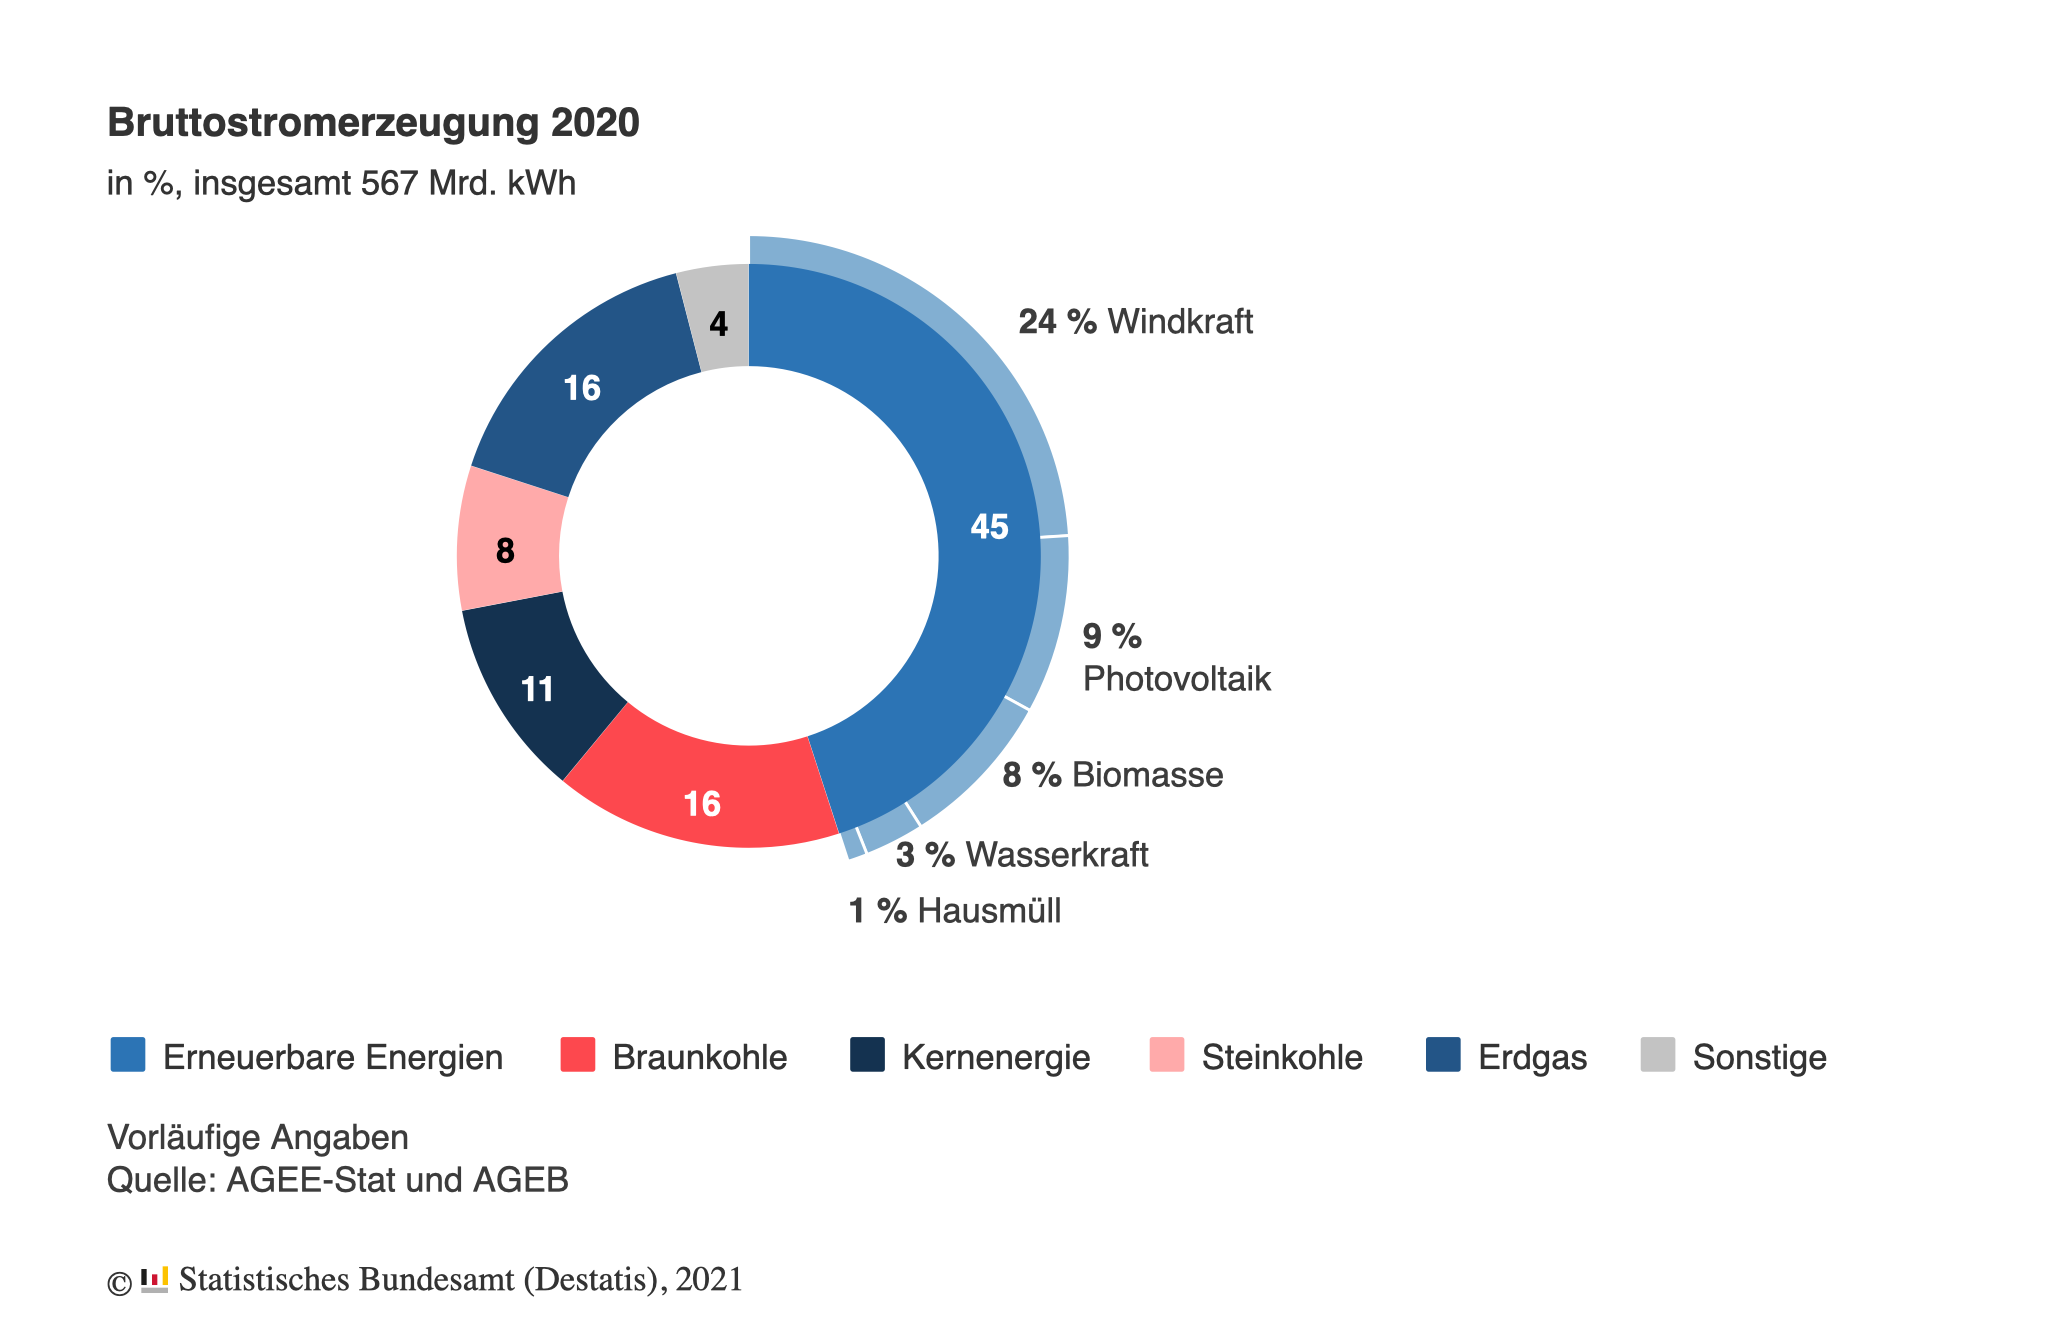
\includegraphics[width=.8\textwidth]{./images/bruttostromerzeugung-erneuerbare-energien.png}
		\caption{Bruttostromerzeugung im Jahr 2020 in Deutschland \cite{2020__Bruttostromerzeugung2020}}
		\label{fig:strommix_deutschland}
	\end{center}
\end{figure}
%%%%%BILD ENDE

Durch eine Überwachung der Windgeschwindigkeit und der Umgebungstemperatur kann daraus die zulässige Übertragungskapazität ermittelt werden. 
Leiterseile halten bei hoher Windgeschwindigkeit und gleichzeitig niedrigen Temperaturen höhere Belastungen aus. 
Es kann also mehr Strom übertragen, wenn mehr Windstrom erzeugt wird \cite{2015_Axthelm_BisFaktenZur}. Aus diesem Grund ist es von großem Interesse Vorhersagen über die Windgeschwindigkeit treffen zu können, um 
die Nutzung des Stromnetzes zu optimieren. In dieser Seminararbeit soll ein Modell entwickelt werden, das 
Windgeschwindigkeit und -richtung eine bis 24 Stunden im Voraus vorhersagen kann. Es sollen in dieses Modell neben zeitlich diskretisierten 
meteorologischen Daten auch eine örtliche Diskretisierung einfließen, welche in dieser Arbeit validiert werden soll.

\section{Einordnung in die Literatur}\label{section:literatur}

In der bestehenden Literatur im Bereich der Windgeschwindigkeits-, beziehungsweise Wettervorhersage, ist eine Entfernung von 
deterministischen Modellen \cite{1963_Lorenz_DeterministicNonperiodicFlow} hin zu Zeitreihenanalyse auf Basis historischer Messdaten erkennbar. 
Innerhalb der letzten zwei Dekaden sind einige Ansätze in der Zeitreihenanalyse zu differenzieren. Klassische Methoden in der 
Zeitreihenprognose, wie das autoregressive moving average (ARMA) und autoregressive integrated moving average (ARIMA) Modell \cite{2016_Cadenas_WindSpeedPrediction} oder auch 
die Weiterentwicklung dessen, mit Berücksichtigung eines saisonalen Einflusses, das saisonale ARIMA (SARIMA) Modell \cite{2018_Alencar_HybridApproachCombining,2019_TenaGarcia_ForecastDailyOutput,2019_Haddad_WindSolarForecasting,2002_Igboekwe_StochasticSimulationHourly,2012_MuhammadSami_PredictionRateDust,
2010_Meng_ModelingForecastingHourly,
2020_Kreuzer_ShorttermTemperatureForecasts} sind 
nicht nur ein häufig verwendetes Vorhersagemodell, sondern werden gerade deshalb auch häufig als Vergleichsmodell herangezogen \cite{2012_Cao_ForecastingWindSpeed,2019_Chen_MultifactorSpatiotemporalCorrelation,2020_Kreuzer_ShorttermTemperatureForecasts}. Darüber hinaus existieren Vektorautoregressive Modelle (VAR)\cite{2014_Orpia_TimeSeriesAnalysis, 2007_Ewing_TimeSeriesAnalysis,2015_He_SparsifiedVectorAutoregressive,2016_Koivisto_WindSpeedModeling, 2015_Dowell_SpatiotemporalPredictionWind}, 
welche im Gegensatz zu ARMA-Modellen mehrere Variablen besitzen. Auch wird es versucht das ARIMA-Modell mit Clustermethoden 
zu verbessern oder mit klassischen Machine Learning Konzepten zu kombinieren \cite{2017_Zhang_HybridMethodShortTerm,2011_Guo_CorrectedHybridApproach}. 
Zunehmend werden auch Neuronale Netze, welche in letzter Zeit stark an Popularität zugenommen haben, für Problemstellungen dieser 
Art verwendet. Neben Ansätzen basierend auf einfachen vorwärtsgerichteten Neuronalen Netzen \cite{2019_Samet_EvaluationNeuralNetworkbased,2017_Chang_ImprovedNeuralNetworkbased}, Convolutional Neural Networks (CNN) \cite{2020_Zhao_ShorttermAverageWind,2019_Chen_MultifactorSpatiotemporalCorrelation},  
Generative Modelle \cite{2019_Khodayar_IntervalDeepGenerative} und Evolutionäre Modelle \cite{2012_Wang_ShorttermWindSpeed} 
waren Ansätze, die auf Recurrent Neural Networks (RNN) basieren auffällig oft vertreten. Hierbei waren RNNs mit Long- Shortterm Memory Units (LSTM) \cite{2018_Dong_WindPowerPrediction,2020_Delgado_WindTurbineData,2020_Moharm_WindSpeedForecast,2019_Prabha_WindSpeedForecasting,2019_Cali_ShorttermWindPower} oder auch LSTM Zellen in Kombination mit 
anderen Technologien \cite{2019_Chen_MultifactorSpatiotemporalCorrelation,2016_Allende_RecurrentNetworksWind,2018_Liu_WindSpeedForecasting,2018_Yao_MultidimensionalLSTMNetworks} sehr prominent.

Drei dieser Ansätze werden hinsichtlich der Datenbasis, des Modellaufbaus und der Modellgüte näher betrachtet. \citeauthor{2020_Delgado_WindTurbineData} \cite{2020_Delgado_WindTurbineData} und 
\citeauthor{2018_Yao_MultidimensionalLSTMNetworks} \cite{2018_Yao_MultidimensionalLSTMNetworks} verwendeten Daten eines Standorts in je der Nordtürkei und Westchina in Intervallen von 
zehn Minuten von je einem Jahr und drei Jahren. \citeauthor{2020_Delgado_WindTurbineData} versuchte mithilfe der generierten Leistung einer Windturbine, der theoretischen Leistung,  
der gemessenen Windgeschwindigkeit und Windrichtung diese vier Parameter der darauf folgenden 10 Minuten zu prognostizieren. Dagegen floss in 
das von \citeauthor{2018_Yao_MultidimensionalLSTMNetworks} entwickelte Modell statt der Leistung der Windturbine die Temperatur ein. \citeauthor{2019_Chen_MultifactorSpatiotemporalCorrelation} 
\cite{2019_Chen_MultifactorSpatiotemporalCorrelation} verwendete Messdaten eines halben Jahres in fünfminütigen Intervallen aus der Region Texas in den USA. 
Es wurden hierbei jedoch nicht nur deutlich mehr unterschiedliche Kenngrößen (Windgeschwindigkeit, Windrichtung, Temperatur, Taupunkt, Temperatur, Windböen, Messhöhe und relative Luftfeuchtigkeit) 
als in den anderen beiden Ansätzen verwendet, sondern auch eine Mehrzahl an Standorten.

Bei dem Modell nach \citeauthor{2020_Delgado_WindTurbineData} handelt es sich um ein RNN mit 65 LSTM Zellen. Die Lossfunktion ist der Mean Absolute Error (MAE), der 
verwendete Optimizer lautet Adam und die Batch Size beträgt 15. Insgesamt wurden 21 Epochen durchlaufen. Es wurde das Single Step Verfahren verwendet. Für die Ergebnisse, monatliche Mittelwerte, dieses Modells wurden der MAE, 
Mean Square Error (MSE) und das Bestimmtheitsmaß ($R^2$) ermittelt. Der MAE der Windgeschwindigkeit liegt in einem Bereich von 0.015m/s bis 0.027m/s. Diese sehr geringen Werte stammen 
mutmaßlich daher, dass in diesem Modell sehr kleine Intervalle der Eingangsdaten mit einer Single Step Prognose kombiniert wurden. 

Im Modell von \citeauthor{2018_Yao_MultidimensionalLSTMNetworks} wurde bei den Eingangsdaten zunächst eine Fuzzy-rough set Faktorreduktion (FRS) durchgeführt. Das RNN, in das die vorverarbeiteten Daten 
einfließen ist folgendermaßen aufgebaut. Das Netz hat drei Layer mit 108 LSTM Zellen und arbeitet mit der Aktivierungsfunktion RELU. Das Modell führt im Gegensatz zum vorherigen beschrienen Modell eine 
rolling prediction durch. Der Input sind jeweils die Daten von zehn Tagen, womit eine Vorhersage von 24 Stunden in die Zukunft getroffen werden soll. 
Eine Cut-off Rate von 0.2 wurde verwendet und die Learning Rate beträgt 0.001. Verwendet wurde der Optimizer RMSprop und das Fehlermaß waren der MAE und der Mean Average Percentage Error (MAPE). 
Um das Modell zu vergleichen wurden neben dem entwickelten Modell dasselbe ohne vorherige Faktorreduktion der Daten und ein Neuronales Netz, welches als Lernverfahren Back Propagation verwendet, entwickelt. 
Aus den Ergebnissen dieser drei Modelle wurden der MAE, MAPE und der maximale Fehler berechnet. Das entwickelte Modell schnitt in diesem Vergleich am besten ab. Im Vergleich zum vorigen Modell ist der MAE höher, 
wobei eine mittlere Abweichung von ungefähr 0.5m/s vertretbar ist.

Das Modell von \citeauthor{2019_Chen_MultifactorSpatiotemporalCorrelation} ist für diese Seminararbeit besonders interessant. Der Einfluss mehrerer Standorte auf die Prognose der Windgeschwindigkeit eines Standorts ist neuartig. 
Um die örtliche mit der zeitlichen Diskretisierung in den Eingabedaten zu verknüpfen und darüber hinaus Informationen über die Korrelation zwischen Zeit, Ort und Naturphänomen herzustellen, wurden die Messdaten mithilfe 
des Mathematical representation of multi factor spatio-temporal correlation model (MFSTC) in einer 3D-Matrix dargestellt. Diese Werte werden von einem CNN mit LSTM Zellen verarbeitet. Das Netz hat eine Batch Size von 128, einen 
Regularisierungskoeffizient von 0.34 und eine Learning Rate von 0.3. 2000 Epochen wurden insgesamt durchlaufen. Verwendet wurde der Optimizer Adam und die Lossfunktion war der MSE. Der Vergleich der Ergebnisse und die Einordnung dieser 
im Vergleich zu anderen Modellen war in dieser Arbeit sehr ausführlich. In drei Experimenten mit jeweils unterschiedlichen Testdaten wurden acht Fehlermaße von variiernden Modellen verglichen. Die Fehlermaße sind die Residuenquadratsumme (SSE), 
der MAE, der RMSE, der Sub-Divisional Error (SDE), der Theilsche Projektionskoeffizient (U1), der Index of agreement (IA), die Direction accuracy (DA) und zuletzt der Pearson correlation coefficient (PCC). Das erste Experiment zielte darauf ab 
die Sinnhaftigkeit der Verwendung des MFSTC Modells und daraufhin die Kombination eines CNNs mit LSTM Zellen mit vorheriger Anwendung des MFSTC Modells zu validieren. Hierbei wurden zunächst ein CNN ohne LSTM Zellen, dasselbe mit Anwendung des 
MFSTC Modells, ein CNN mit LSTM Zellen und das entwickelte Modell verglichen um MFSTC zu validieren und im Anschluss ein CNN ohne LSTM Zellen, mit LSTM Zellen, ein MFSTC-CNN ohne LSTM Zellen und das entwickelte Modell verglichen. 
Im zweiten Teil des ersten Experiments wurden ein ARIMA Modell und ein Multi Layer Perceptron (MLP) zusätzlich als Benchmark verwendet. Das entwickelte Modell schnitt im Vergleich zu den anderen Modellen am besten ab, womit die Sinnhaftigkeit der Verwendung des 
MFSTC Modells und auch des entwickelten Modells validiert werden konnten. Der MAE des Modells war in einem Bereich von 1m/s. 
Im zweiten Experiment wurden nun einige unterschiedliche Neuronale Netze miteinander verglichen. Neben einer Linearen Regression (LR), einem MLP, einem CNN, einem LSTM und einer Kombination aus dem MFSTC Modell mit einer CNN-MLP Fusion und MLP-LSTM Fusion, 
schnitt das von \citeauthor{2019_Chen_MultifactorSpatiotemporalCorrelation} entwickelte Modell wieder am besten ab. Der MAE war nun im Bereich von 2m/s. 
Das dritte Experiment verglich nun das eigene Modell mit üblichen Modellen der Windprognose und den Modellen von drei anderen Veröffentlichungen. Wieder schnitt das entwickelte Modell am besten ab. 
Zuletzt wurde mit all den erhaltenen Ergebnissen der Diebold-Mariano Test durchgeführt, eine übliche Hypothesen Testmethode, bei der die Tauglichkeit des vorgestellten Modells gegenüber den anderen Methoden endgültig validiert wird.

Anhand dieser drei vorgestellten Paper ist erkenntlich, dass Windprognosemodelle, die dem Stand der Technik entsprechen, nicht nur eine stark voneinander abweichende Datenbasis besitzen, sondern auch die Modelle, die sich alle der Technologie von LSTM Zellen 
zu Nutze machen, trotzdem stark voneinander abweichen. Aufgrund dieser großen Vielfalt an Freiheitsgraden ist die Validierung und Einordnung von Windprognosemodellen sehr komplex und in der vorhandenen Literatur keinesfalls einheitlich.

\section{Ziele dieser Arbeit}

Wie bereits in Kapitel \ref{section:einleitung} angemerkt, wird in dieser Seminararbeit das Ziel verfolgt ein Prognosemodell, welches Windgeschwindigkeit und Windrichtung mit ausreichender Qualität vorhersagen kann, nach dem jetzigen Stand der Technik zu entwickeln. 
In Kapitel \ref{section:literatur} stellt sich heraus, dass sich die Methodik der Windprognose im Laufe der Zeit zur Verwendung von Deep Neural Networks entwickelt hat. Der Großteil dieser Ansätze, welcher elf von 16 entspricht, basiert auf Recurrent neural networks (RNN) mit Long short-term memory units (LSTM). 
Aufgrunddessen und da diese Veröffentlichungen auch die vielversprechendsten Ergebnisse liefern, soll das in dieser Arbeit vorgestellte Prognosemodell auf Basis dieser Technologie entwickelt werden. 
Im Laufe der Literaturrecherche haben sich zudem noch zwei weitere Fragen aufgetan, welche anhand des entwickelten Modells beantwortet werden sollen. 
Inspiriert durch das von \citeauthor{2019_Chen_MultifactorSpatiotemporalCorrelation}\cite{2019_Chen_MultifactorSpatiotemporalCorrelation} Modell, welcher nicht nur einen, sondern Messdaten mehrerer Standorte berücksichtigte, stellte sich folgende Frage. 
Hat die Berücksichtigung mehrerer unmittelbar umliegender Standorte einen positiven Einfluss auf die Ergebnisse des Vorhersagemodells? 
Des weiteren stellte sich heraus, dass in den meisten in Kapitel \ref{section:literatur} beschriebenen Papern ausschließlich die Windgeschwindigkeit vorhergesagt wird und die Windrichtung nicht in die Vorhersage einfließt, beziehungsweise nicht vorhergesagt wird. 
In dieser Arbeit sollen Windgeschwindigkeit und Windrichtung prognostiziert werden, wobei Windrichtung und -geschwindigkeit als Vektor unterschiedlich dargestellt werden können. 
Hierbei stellt sich die Frage, ob in den Ergebnissen der Windprognose eine Verbesserung erkennbar ist, wenn die Windvektor nicht mit Polarkoordinaten, sondern stattdessen mit kartesischen Koordinaten beschrieben wird? 
Im Laufe dieser Arbeit werden der Aufbau des Prognosemodells mitsamt seiner Besonderheiten beschrieben und dessen Ergebnisse diskutiert und eingeordnet. 
Die Fragen, welche innerhalb dieses Abschnittes beschrieben wurden, sollen daraufhin im Rahmen von Versuchen mithilfe des entwickelten Modells beantwortet werden.

%%%%%%%%%%%%%%%%%%%%%%%%%%%%%%%%%%%%%%%%%%%%%%%%%%%%%%%%%%%%%%%%%%%%%%%
%                                                                     %
%                                                                     %
%                                                                     %
%                               KAPITEL                               %
%                                                                     %
%                                                                     %
%                                                                     %
%%%%%%%%%%%%%%%%%%%%%%%%%%%%%%%%%%%%%%%%%%%%%%%%%%%%%%%%%%%%%%%%%%%%%%%
\chapter{Grundlagen}
Dieses Kapitel soll die Grundlagen von Neuronalen Netzen, insbesondere die Funktionsweise von RNNs und von LSTM Zellen, vermitteln, da auf diesen Technologien das vorgestellte Windprognosemodell basiert. 
Darüber hinaus wird beschrieben um was es sich bei zirkulären Daten handelt und was diese im Rahmen von neuronalen Netzen für Herausforderungen darstellen können.

\section{Neuronale Netze zur Zeitreihenprognose}

Ein künstliches neuronales Netz ist klassischer Weise in Schichten (Layers) aufgebaut. Jede Schicht besteht aus mindestens einem, meistens aber vielen Neuronen. Bezeichnet werden die Schichten Input-, Hidden- und Output-Layer. In Abbildung \ref{fig:nn} ist ein solches neuronales Netz schematisch dargestellt.

%%%%%BILD ANFANG
\begin{figure}[tph]
	\begin{center}
		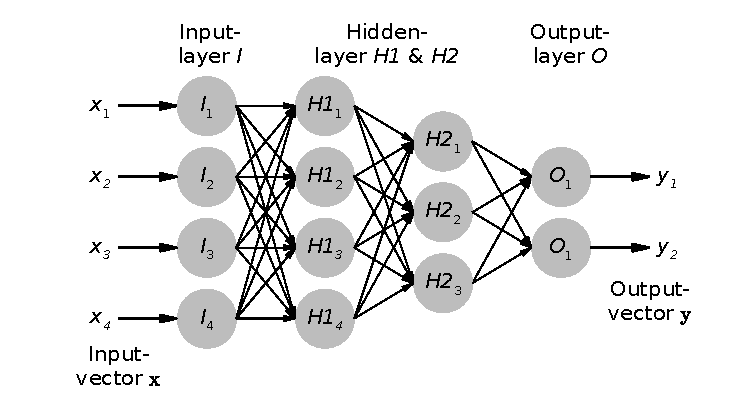
\includegraphics[width=0.6\linewidth]{./images/knn_allg.pdf}
		\caption{Schematische Darstellung eines klassischen neuronalen Netzes}
		\label{fig:nn}
	\end{center}
\end{figure}
%%%%%BILD ENDE

Neuronen zwischen zwei Schichten sind durch gewichtete Verbindungen miteinander verknüpft. Die Gewichte aller Verbindungen sind die \qm{Stellschrauben} des neuronalen Netzes. In diesen ist die Fähigkeit der Vorhersage codiert. Im Lernprozess werden diese Gewichte sukzessive geändert.

Ein Neuron besitzt im Allgemeinen mindestens eine Eingabe und genau eine Ausgabe, wobei diese als die Aktivität des Neurons bezeichnet wird. Die Eingaben entsprechen den gewichteten Verbindungen zu den Vorgängerneuronen. Die Summe aller Eingaben wird zusammen mit dem sogenannten Bias (Trainierbarer Parameter pro Neuron, der einen Offset der summerten Eingabe ermöglicht.) über die Aktivierungsfunktion in die Aktivität des Neurons umgewandelt. 

Die Eingabedaten werden dem neuronalen Netz durch den Input-Vektor $\mathrm{x}$ präsentiert und durch das Netz propagiert. Die Aktivitäten der Neuronen in der Output-Layer werden im Output-Vektor $\mathrm{y}$ gesammelt. Dieser Vektor gleicht dem Prognoseergebnis. Im Trainingsprozess wird der Output-Vektor mit dem zu erwartenden Ergebnis verglichen. Der Fehler zwischen Prognose und dem erwarteten Ergebnis wird durch das neuronale Netz zurück propagiert. Dabei werden die Gewichte der Verbindungen so angepasst, dass der ermittelte Fehler verringert wird (sog. Backpropagation). 

RNN
LSTM, insbesondere Vor und Nachteile

\highlight{ein paar Grundlagen zu neuronalen Netzen; 
Beschreibung NN allgemein, RNN, LSTM Zellen und warum gut für Prognose}


%%%%%BILD ANFANG
\begin{figure}[tph]
	\begin{center}
		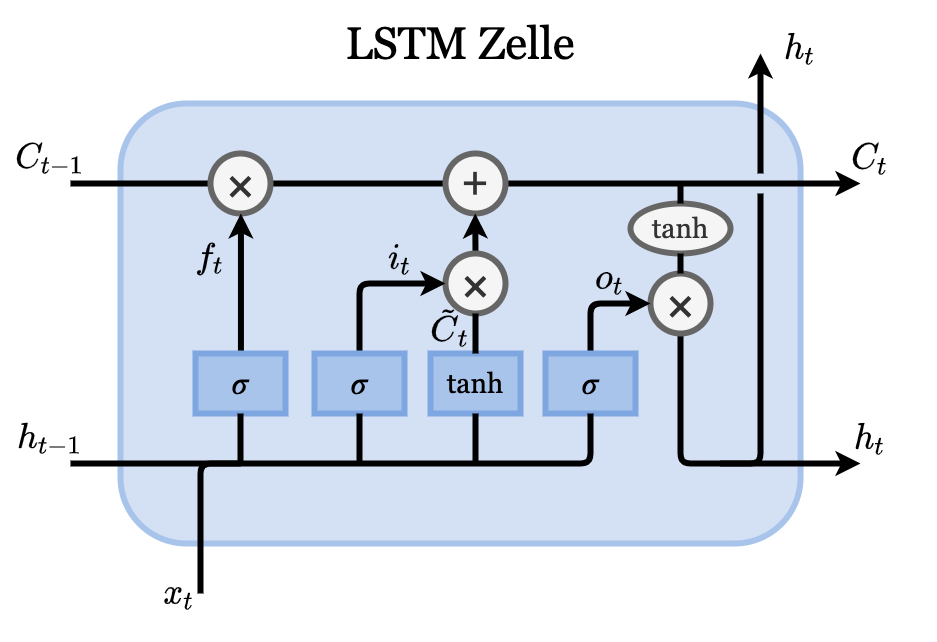
\includegraphics[width=0.5\linewidth]{./images/LSTM_Zelle.png}
		\caption{Schematische Darstellung einer LSTM Zelle}
		\label{fig:lstm}
	\end{center}
\end{figure}
%%%%%BILD ENDE

\newpage

\section{Zirkuläre Daten}\label{section:circ_data}

Wird in dieser Seminararbeit von zirkulären Daten gesprochen, sind Datensätze gemeint, welche sich für den Menschen intuitiv in einem Kreis anordnen lassen. 
Hierzu gehören beispielsweise die Himmelsrichtungen auf einem Kompass, der Farbton dargestellt als Winkel (siehe Abbildung \ref{fig:colorcircle}), der Längengrad entlang des Äquators, die Rotation eines Objekts im Raum oder auch zyklische Daten, wie die Sekunden, Minuten und Stunden auf der Uhr \cite{2016_London_EncodingCyclicalContinuous}. 
All diese Daten haben gemein, dass bei einer quantitativen Beschreibung in einem Punkt des Kreises der geringste Wert aufgetragen wird, die Werte entlang dessen Linie aufsteigen und schließlich einen Punkt vor dem Anfangspunkt mit dem höchsten Wert enden. 
Hierbei passiert nun das Phänomen, dass der objektiv betrachtet höchste und niedrigste Wert dieser Skala, also die Werte, welche mathematisch am weitesten voneinander entfernt liegen, in Wahrheit inhaltlich viel stärker miteinander verknüpft sind als diese mit 
einem mathematisch näher liegenden Wert aus der Mitte. 

%%%%%BILD ANFANG
\begin{figure}[tph]
	\begin{center}
		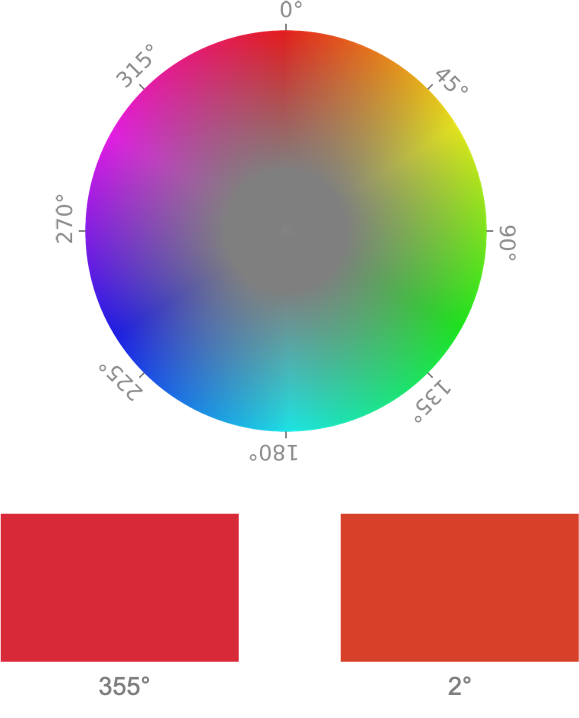
\includegraphics[width=0.5\linewidth]{./images/colorcircle.png}
		\caption{Darstellung des Farbtons mit Winkelangaben, sowie zwei Rottöne mit ihrer Winkelbezeichnung \cite{__Farbraum}}
		\label{fig:colorcircle}
	\end{center}
\end{figure}
%%%%%BILD ENDE

Beispielhaft ist eine Farbe im Farbkreis (siehe Abbildung \ref{fig:colorcircle}), die mit einem Winkel von $2^\circ$ beschrieben wird für den Betrachter rot und eine mit $90^\circ$ beschriebene Farbe als grün erkennbar. Die mit $355^\circ$ beschriebene Farbe, die einen 
vier Mal größeren Abstand zur roten Farbe hat wie die rote Farbe zur grünen Farbe, ist jedoch auch rot und kaum von der ersten Farbe zu unterscheiden. 
Dieser für den Menschen intuitive Zusammenhang geht in der herkömmlichen Darstellung, das sind Gradangaben oder übliche Zeitangaben, verloren \cite{2016_London_EncodingCyclicalContinuous}. 
Gerade im Zusammenhang mit Neuronalen Netzen ist es jedoch sehr wichtig diesen zirkulären Gedanken in den Eingabedaten zu erhalten, damit Korrelationen zwischen Größen besser verstanden werden. 
Ein Ansatz dieses Problem zu umgehen ist es die Daten so zu transformieren, dass die zirkuläre Information erhalten bleibt. Im Laufe dieser Arbeit werden zwei Transformationen vorgestellt, die zeitliche (vgl. Kapitel \ref{section:gen_daten}) und räumliche (vgl. Kapitel \ref{section:Winddaten_vec}) Daten so verändern wollen, dass sie für ein Neuronales Netz besser zu verstehen sind.

%%%%%%%%%%%%%%%%%%%%%%%%%%%%%%%%%%%%%%%%%%%%%%%%%%%%%%%%%%%%%%%%%%%%%%%
%                                                                     %
%                                                                     %
%                                                                     %
%                               KAPITEL                               %
%                                                                     %
%                                                                     %
%                                                                     %
%%%%%%%%%%%%%%%%%%%%%%%%%%%%%%%%%%%%%%%%%%%%%%%%%%%%%%%%%%%%%%%%%%%%%%%

\chapter{Daten}

Für eine Prognose von Winddaten mithilfe von Technologien des Deep learning werden Messdaten aus der Vergangenheit benötigt. 
In den folgenden Unterkapiteln wird beschrieben woher die letztlich verwendeten Daten stammen und wie diese Daten verarbeiten werden müssen, um für Prognosen verwendet werden zu können.

\section{Datenbasis}\label{section:datenbasis}
Zur Erstellung des Modells wurde eine Kombination aus gemessenen Daten von Stationen des Deutschen Wetterdienstes (DWD) sowie künstlich generierten Daten verwendet.
Während die gemessenen Daten die aktuelle Wetterlage an einigen Standorten Deutschlands beinhalten, geben die generierten Daten darüber hinaus weitere Informationen zu saisonalen und täglichen Abhängigkeiten. Die Zusammensetzung des Rohdatzensatzes kann der Abbildung \ref{fig:rohdatensatz} entnommen werden. Nach der in Kapitel \ref{section:Datenaufbereitung} beschriebenen Datenaufbereitung kann dieser Datensatz zum Training des neuronalen Netzes genutzt werden.

%%%%%BILD ANFANG
\begin{figure}[tph]
	\begin{center}
		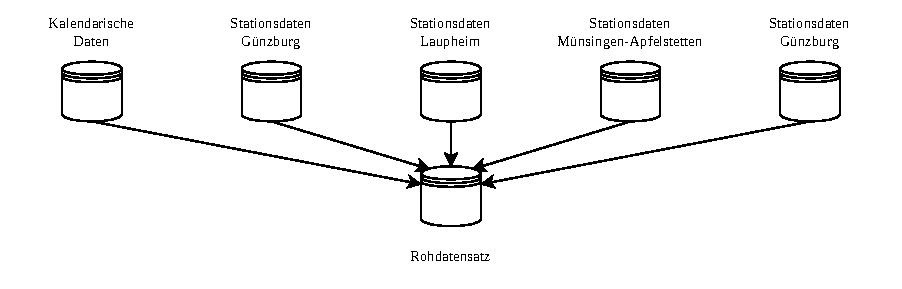
\includegraphics[]{./images/rohdatensatz.pdf}
		\caption{Zusammensetzung des Rohdatensatzes}
		\label{fig:rohdatensatz}
	\end{center}
\end{figure}
%%%%%BILD ENDE

\subsection{Reale Messdaten}\label{section:realeMessdaten}
Die realen Messdaten werden vom Deutschen Wetterdienst über einen Webserver kostenlos zur Verfügung gestellt. In dieser Arbeit sind die Daten in stündlicher Auflösung von vier Messtationen (Münsingen-Apfelstetten, Stötten, Günzburg und Laupheim) im Ulmer Umkreis zum Einsatz gekommen. Die genaue geographische Lage kann der Abbildung \ref{fig:map} entnommen werden. Der Deutsche Wetterdienst betreibt im Ulmer Umkreis zwar noch weitere Wetterstationen, jedoch messen diese die Windgeschwindigkeit und Windrichtung nicht. Insgesamt umfasst der Datensatz den Zeitraum Anfang 2016 bis Ende 2021. Davon sind jedoch rund $20\%$ Datenlücken (Genaue Darstellung siehe Heatmap \ref{fig:heatmap}). Diese werden in Kapitel \ref{section:Datenlücken} genauer beleuchtet. 

%%%%%BILD ANFANG
\begin{figure}[tph]
	\begin{center}
		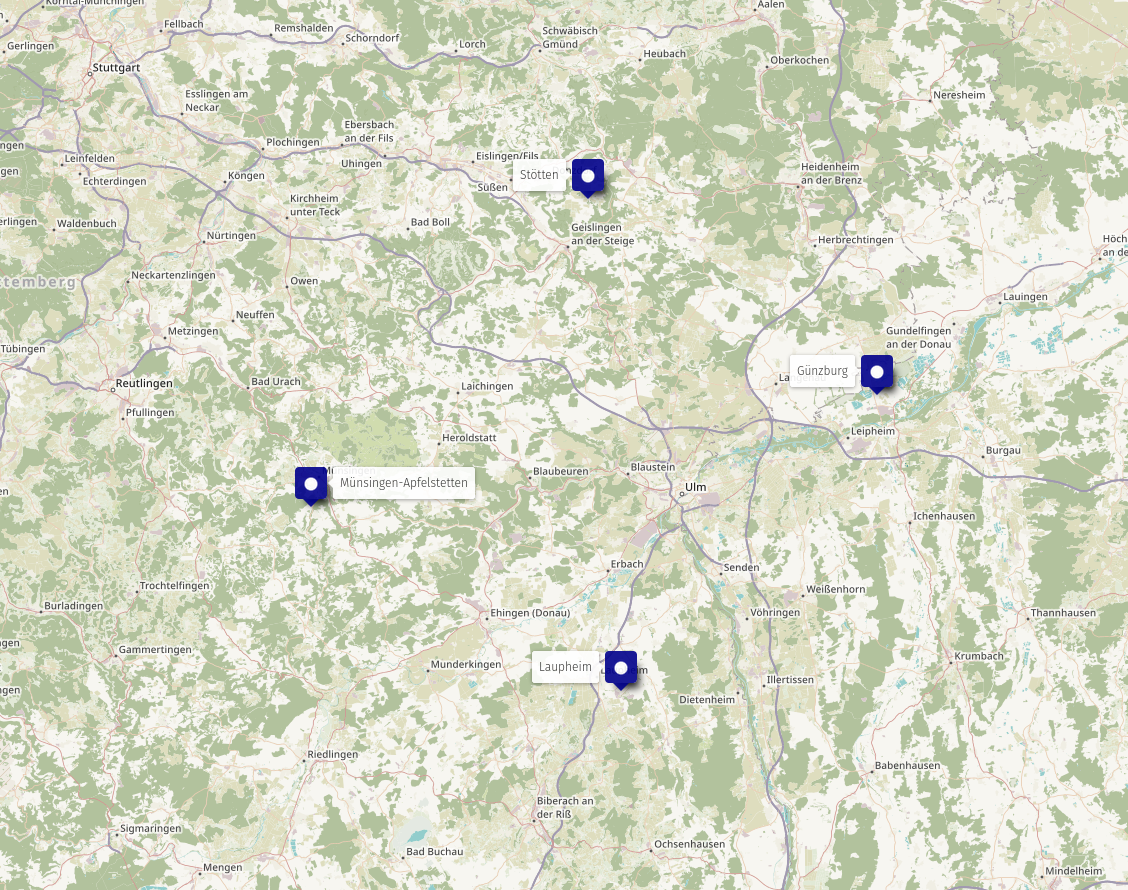
\includegraphics[width=\textwidth]{./images/map.png}
		\caption{Geographische Lage der Messstationen \cite{2021_OpenStreetMap-Contributors_UMap}}
		\label{fig:map}
	\end{center}
\end{figure}
%%%%%BILD ENDE

%%%%%BILD ANFANG
\begin{figure}[tph]
	\begin{center}
		\includegraphics[width=\linewidth]{./images/Datenausfälle_all-cropped.jpg}
		\caption{Heatmap der Datenausfälle aller Datenreihen, wobei rot einen solchen kennzeichnet. Zu beachten ist, dass durch die Bildauflösung nur Datenausfälle von mehr wie $~40h$ dargestellt werden können.}
		\label{fig:heatmap}
	\end{center}
\end{figure}
%%%%%BILD ENDE

Zur Prognose der Windgeschwindigkeit und Windrichtung können neben deren selbst auch andere Messgrößen wie Sonnenscheindauer, Luftdruck, Temperatur und Luftfeuchtigkeit genutzt werden. Jedoch wird nicht jede dieser Größen an jeder Messstation bestimmt. Die folgende Tabelle \ref{tab:messgrößen} gibt einen detaillierteren Aufschluss über die tatsächlich gemessenen Größen.

%%%%%TABELLE ANFANG
\begin{table}[tph]
	\centering
	\caption{Gemessene Größen je Messstation}
	\begin{tabular}{|l|c|c|c|c|c|}
		\hline
        \rowcolor{color80}
		& \textbf{Auflösung} & \textbf{\makecell{Münsingen-\\ Apfelstetten}} & \textbf{Stötten} & \textbf{Günzburg} & \textbf{Laupheim} \\\hline
		Windgeschwindigkeit & $0.1m/s$ & \cmark & \cmark & \cmark & \cmark \\\hline
		Windrichtung & $10^\circ$ & \cmark & \cmark & \cmark & \cmark \\\hline
		Sonnenscheindauer & $1min$ & \cmark & \cmark & \xmark & \xmark \\\hline
		Luftdruck & $0.1hPa$ & \xmark & \cmark & \xmark & \cmark \\\hline
		Temperatur & $0.1^\circ C$ & \cmark & \cmark & \cmark & \cmark \\\hline
		Luftfeuchtigkeit & $1\%$ & \cmark & \cmark & \cmark & \cmark \\\hline
	\end{tabular}
\label{tab:messgrößen}
\end{table}
%%%%%TABELLE ENDE

Um einen tieferen Einblick in das Verhalten des Windes an der jeweiligen Messstation zu erhalten, bieten sich Windrosen zur Visualisierung an. Dabei wird die Häufigkeit der Windgeschwindigkeit in Abhängigkeit der Windrichtung radial dargestellt. Der Abbildung \ref{fig:windroses} können die Windrosen für die vier ausgewählten Messstationen entnommen werden. Wie in den südlichen Regionen Deutschlands zu erwarten, ist die vorherschende Windrichtung West bis Südwest. 

Bei detaillierter Analyse fällt jedoch auf, dass der Wind an der Messstation Münsingen- Apfelstetten besonders bei leichtem Wind sehr volatil ist. Der Grund hierfür könnte in der Tatsache begründet sein, dass sich die Messstation in einem flachen Tal mit Nord-Südlicher Ausrichtung befindet. Des Weiteren ist zu erkennen, dass unter den vier Messstationen in Stötten die stärksten Winde auftreten. In dieser Arbeit wird die Windgeschwindigkeit für die Messstation in Günzburg prognostiziert. 

%%%%%BILD ANFANG
\begin{figure}[tph]
	\begin{center}
		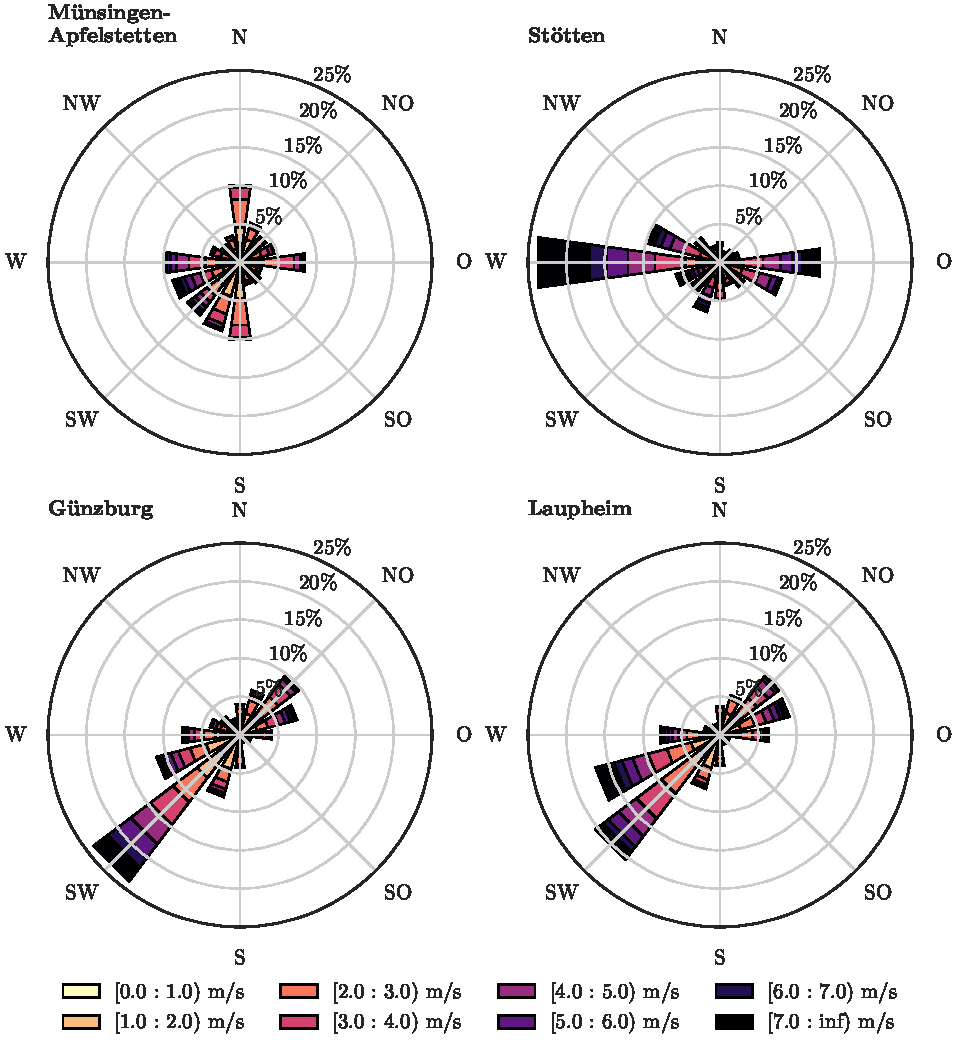
\includegraphics[width=0.9\linewidth]{./images/windroses.pdf}
		\caption{Windrosen der vier ausgewählten Messstationen}
		\label{fig:windroses}
	\end{center}
\end{figure}
%%%%%BILD ENDE



\subsection{Generierte Messdaten}\label{section:gen_daten}
Die Wetterlage in Deutschland weist wiederkehrende Trends innerhalb eines Tages und auch innerhalb eines Jahres auf. Offensichtlich ist es am Tag wärmer als in der Nacht und im Sommer wärmer als im Winter. Um diese Information für das Modell nutzbar zu machen, werden zusätzlich zu den gemessenen Daten zwei weitere Variablen eingeführt, nämlich die Tageszeit und die Jahreszeit. 
Die Darstellung von zeitlichen Daten ist jedoch zyklisch. Sowohl Sekunden, Minuten und Stunden, als auch Wochentage und Monate werden beim Überschreiten der oberen Intervallgrenze auf die untere zurückgesetzt. Wie bereits in Kapitel \ref{section:circ_data} betont, müssen diese Daten so transformiert werden, das das Neuronale Netz die Informationen richtig verarbeiten kann.

\begin{itemize}
	\item \textit{Kalendarischer Tageswert}\\
	Über die folgende Funktion wird die Stunde des Tages $HOD \in [0, \dots, 23]$ in einen Sinuswelle umgewandelt. Das Maximum wird um 12 Uhr, das Minimum um 0 Uhr erreicht. Abgebildet wird auf das Intervall $[0,1]$.
	
	\begin{equation}\label{eq:cal_day}
		cal_{day} = \frac{1}{2}\Big(\cos \big(\pi (\frac{HOD}{12}+ 1)\big) + 1 \Big)
	\end{equation}

	%%%%%BILD ANFANG
	\begin{figure}[tph]
		\begin{center}
			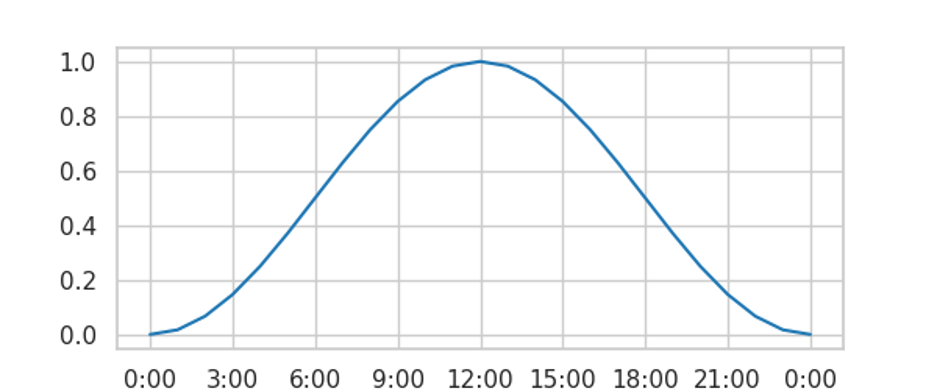
\includegraphics[]{./images/sinuszeit.png}
			\caption{Visualisierung der Sinusfunktion \ref{eq:cal_day}}
			\label{fig:sinustag}
		\end{center}
	\end{figure}
	%%%%%BILD ENDE
	
	\item \textit{Kalendarischer Saisonalwert}\\
	Die folgende Funktion transformiert den Tag des Jahres $DOY \in [1, \dots, 365]$ in eine Sinuswelle. Schaltjahre werden nicht berücksichtigt. Außerdem wird die Stunde des Tages $HOD \in [0, \dots, 23]$ mit einbezogen. Diese spielt für den Funktionswert jedoch nur eine untergeordnete Rolle. Das Maximum wird am 1.Juli, das Minimum am 1.Januar erreicht. Die Funktion bildet ebenfalls auf das Intervall $[0,1]$ ab.
	\begin{equation}\label{eq:cal_seas}
		cal_{seas} = \frac{1}{2}\Big(\cos\big(\pi (\frac{DOY -1 + \frac{HOD}{24}}{\frac{365}{2}}+ 1)\big) + 1\Big)
	\end{equation}
	
	%%%%%BILD ANFANG
	\begin{figure}[tph]
		\begin{center}
			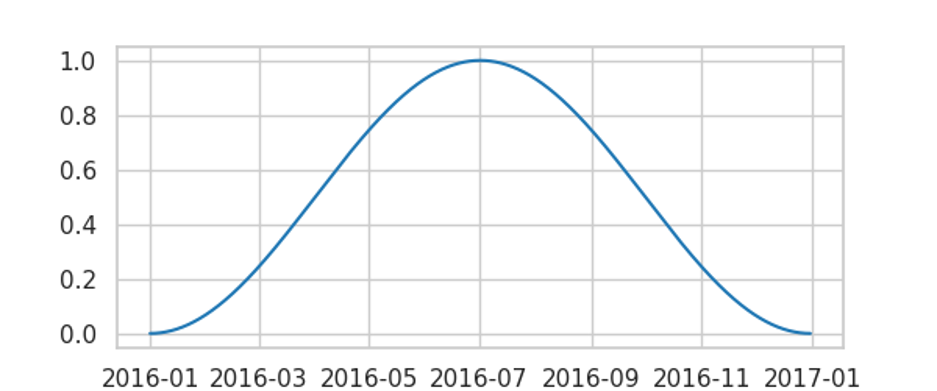
\includegraphics[]{./images/sinusdatum.png}
			\caption{Visualisierung der Sinusfunktion \ref{eq:cal_seas}}
			\label{fig:sinusjahr}
		\end{center}
	\end{figure}
	%%%%%BILD ENDE

\end{itemize}

Anzumerken ist hierbei, dass diese Formeln keine ideale Repräsentation der Zusammenhänge zwischen einer zeitlichen Komponente mit der Wetterlage darstellt. Beispielsweise ist der wärmste Zeitpunkt eher im August, also einen Monat später, anzusiedeln. Die Tageshöchsttemperaturen weichen sogar noch stärker ab. In den Wintermonaten liegen diese zwischen 13 und 14 Uhr und in den Sommermonaten sogar erst zwischen 16 und 17 Uhr. \cite{2017__WarumIstEs}

Des Weiteren ist die Codierung kalendarischer Daten über diese Methode nicht eindeutig, so gilt z.B. $dal_{day}(HOD=6Uhr) = dal_{day}(HOD=18Uhr)$. Abhilfe könnte hier eine zweite um $\pi/2$ bzw. $6h$ verschobene Sinusfunktion leisten, wodurch der Zeitpunkt eindeutig zugeordnet werden kann. Dies wurde in dieser Arbeit jedoch nicht implementiert.

% \subsection{Analyse der Datenbasis}
% \highlight{Korrelationskoeffizient fand Schlüter nicht so gut}
% Der Korrelationskoeffizient gibt Aufschluss darüber, ob zwischen zwei größen ein linearer Zusammenhang besteht. Er kann als Entscheidungshilfe zur Auswahl der Input-Größen für das neuronale Netz dienen. In Abbildung \ref{fig:corr} wird die Korrelation zwischen den Größen relative Luftfeuchte ($RH$), Sonnenscheindauer ($SD$), Temperatur ($T$), Windgeschwindigkeit ($v$), Windrichtung ($\varphi$) sowie die in Kapitel \ref{section:gen_daten} beschriebenen kalendarischen Daten $cal_{day}$ und $cal_{seas}$ dargestellt. 



% Da die Größen Windstärke und Windrichtung prognostiziert werden sollen, sind die Korrelationen zwischen dieser und anderer Größen natürlich von besonderem Interesse. Aus Abbildung \ref{fig:corr} lässt sich erkennen, dass der Luftdruck in einem Zusammenhang mit der Windgeschwindigkeit steht (Fällt $RH$ steigt $v$). Ebenso lässt sich aus der Korrelation zwischen Windgeschwindigkeit und der Temperatur bzw. dem kalendarischen Saisonalwert $cal_{seas}$ eine erhöhte Windgeschwindigkeit im Winter ablesen. Der kalendarische Tageswert $cal_{day}$ scheint jedoch nicht in einem linearen Zusammenhang mit der Windgeschwindigkeit zu stehen.

% \bigskip
% An dieser Stelle ist es wichtig zu erwähnen, dass der Korrelationskoeffizient nur einen linearen Zusammenhang zwischen zwei größen abbildet. Komplexere Zusammenhänge werden nicht erkannt \cite{2020_Ranjan_EstimatingNonlinearCorrelation}. Es ist also möglich, dass eine Größe für die Prognose wertvolle Information enthält, jedoch nicht mit der Windgeschwindigkeit korreliert.

% %%%%%BILD ANFANG
% \begin{figure}[tph]
% 	\begin{center}
% 		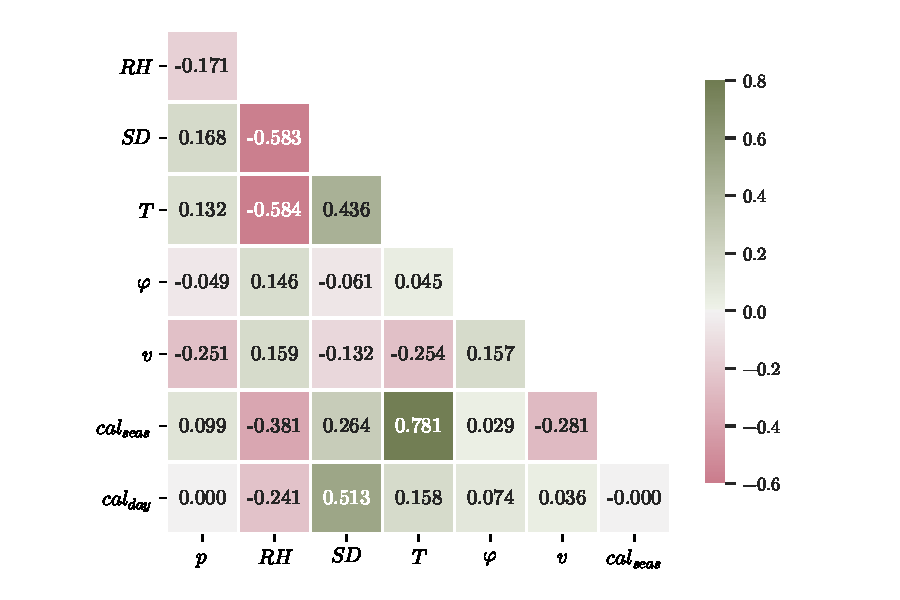
\includegraphics[]{./images/corr.pdf}
% 		\caption{Korrelationskoeffizienten für die Messdaten der Station in Stötten \highlight{(Ändern zu Günzburg, da diese prognostiziert wird)} sowie kalendarische Daten im Zeitraum 01.01.2016 bis 31.12.2020.}
% 		\label{fig:corr}
% 	\end{center}
% \end{figure}
% %%%%%BILD ENDE

\section{Datenaufbereitung}\label{section:Datenaufbereitung}
Die Datenaufbereitung ist häufig eines der aufwendigeren Teile eines Machine-Learning Projektes. Daher wird in dieser Arbeit auf diesen Teil vertieft eingegangen. Abbildung \ref{fig:preprocessing} skizziert den Ablauf der Datenaufbereitung. Dabei werden die folgenden fünf Schritte durchlaufen, die in den nachfolgenden Kapiteln detaillierter beschrieben werden:

%%%%%BILD ANFANG
\begin{figure}[tph]
	\begin{center}
		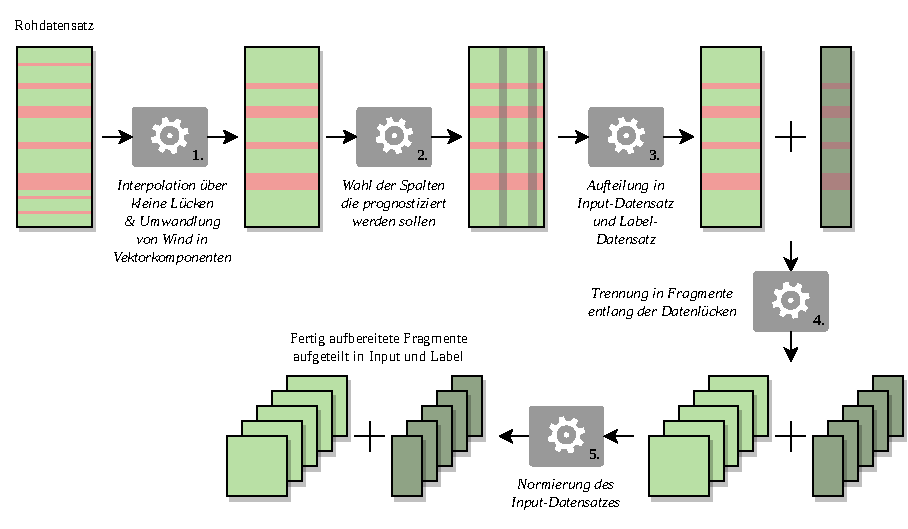
\includegraphics[]{./images/preprocessing.pdf}
		\caption{Ablauf der Datenaufbereitung. Der Datensatz wird vertikal dargestellt, wobei Datenlücken rot sind.}
		\label{fig:preprocessing}
	\end{center}
\end{figure}
%%%%%BILD ENDE

\begin{enumerate}
	\item Im Rohdatensatz gibt es einige kürzere und längere Datenlücken (In Abb. \ref{fig:preprocessing} dargestellt als rote Segmente). Über kurze Datenlücken wird linear interpoliert. Außerdem werden die Winddaten von der polaren in eine kartesische Darstellung umgewandelt.
	\item Aus dem durch Schritt 1. generierten Datensatz werden die Spalten gewählt, die es zu prognostizieren gilt (In Abb. \ref{fig:preprocessing} dargestellt durch verdunkelte Spalten). In dieser Arbeit wird die Windgeschwindigkeit und Windgeschwindigkeit einer Station gewählt.
	\item Der Datensatz wird nun in einen Inputdatensatz und einen Labeldatensatz (In Abb. \ref{fig:preprocessing} verdunkelt) aufgeteilt.
	\item Die verbleibenden längeren Datenlücken im Input- und Labeldatensatz werden \qm{herausgeschnitten}. Übrig bleiben Fragmentpaare, die keine Fehlstellen enthalten.
	\item Der Inputdatensatz (hellgrün) wird normiert. Dieser Schritt erleichtert das Training des neuronalen Netzes.
\end{enumerate}

\subsection{Interpolation über Datenlücken}\label{section:Datenlücken}

In realen Messsystemen kann es immer wieder zu Ausfällen kommen (z.B. vereistes Anemometer oder verschmutzte Sensoren). Auch kann es bei der Übertragung oder Speicherung der Daten zu Fehlern kommen. Der Deutsche Wetterdienst hat daher ein mehrstüfiges Validationssystem und kennzeichnet Fehler entsprechend. In den Rohdaten (siehe Kap. \ref{section:datenbasis}) ist dies meist als Wert $-999$ gekennzeichnet. Es kann sich also darauf verlassen werden, dass die verbleibenden \qm{wahren} Daten glaubhaft sind. 

Datenlücken müssen vor dem Training mit dem neuronalen Netz entfernt werden. In Abhängigkeit der Länge des Zeitraums $\Delta t$, über den sich eine Datenlücke erstreckt, wird die Datenlücke entfernt:

\begin{itemize}
	\item $\Delta t \leq 4h$
	
	Tritt eine kurze Datenlücke auf, so werden die fehlenden Werte durch eine lineare Interpolation anhand der direkt umschließenden wahren Werte ergänzt.

	\item $\Delta t > 4h$

	Eine Interpolation längerer Daten ist nicht mehr sinnhaft. Daher wird der Datensatz, wie in Abbildung \ref{fig:preprocessing} im vierten Schritt verdeutlicht, entlang großer Datenlücken aufgeteilt.

\end{itemize}

\subsection{Winddaten als Vektoren}\label{section:Winddaten_vec}
Die Windmessung erfolgt (von modernen Laser- oder Schallmessungen abgesehen) üblicherweise mithilfe eines Schalenanemometers und einer Windfahne. Zu jedem Messzeitpunkt werden also zwei Werte aufgenommen. Die Windgeschwindigkeit $v$ wird in $m/s$ gemessen. Die Windrichtung $\varphi$ wird typischer Weise in Grad angegeben, es gilt also $\varphi \in [0,360)$. Norden wird dabei mit $\varphi_{north} = 0^\circ$ gewählt. Dieses $(v,\varphi)$-Tupel lässt sich als Polarkoordinate interpretieren. Jedoch tritt hier das in Kapitel \ref{section:circ_data} beschriebene Problem der zirkulären Daten auf, da $\varphi_{north} = 0^\circ = 360^\circ$ gilt.

Es gilt zu belegen, dass sich dieses Problem umgehen lässt, indem der Wind nicht in polaren sondern kartesischen Koordinaten dargestellt wird. Der Windvektor, der durch das $(v,\varphi)$-Tupel beschrieben ist, wird so in eine $v_x$ und eine $v_y$ Komponente zerlegt. Dieses Vorgehen ist in Abbildung \ref{fig:pol2cart} skizziert.

%%%%%BILD ANFANG
\begin{figure}[tph]
	\begin{center}
		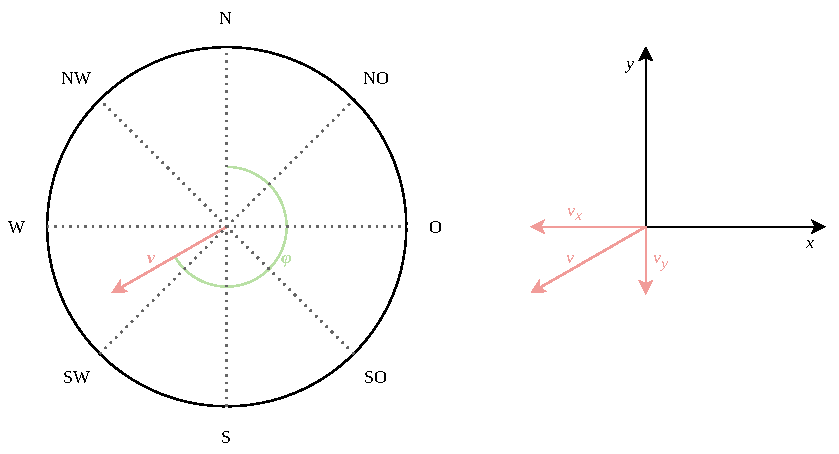
\includegraphics[scale = 1]{./images/pol2cart.pdf}
		\caption{Interpretation der Windgeschwindigkeit und Windrichtung als Vektorkomponenten}
		\label{fig:pol2cart}
	\end{center}
\end{figure}
%%%%%BILD ENDE

Die hier beschriebene Umwandlung kann der Abbildung \ref{fig:pol2cart2} anhand realer Messdaten entnommen werden. Im oberen Teil ist die Häufigkeitsverteilung in $(v,\varphi)$-Form dargestellt. Die zirkuläre Eigenschaft $\varphi_{north} = 0^\circ = 360^\circ$ ist hier nicht sichtbar. Die Häufigkeitsverteilung für die umgewandelten Koordinaten in $(v_x,v_y)$-Form hingegen ist klar um den Ursprung verteilt. Hier lässt sich die zirkuläre Eigenschaft gut erkennen. Das strahlenartige Muster erklärt sich durch die diskrete Angabe der Windrichtung in $10^\circ$ Schritten. Bei einer feineren Auflösung wäre die Verteilung weniger verzerrt.

%%%%%BILD ANFANG
\begin{figure}[tph]
	\begin{center}
		%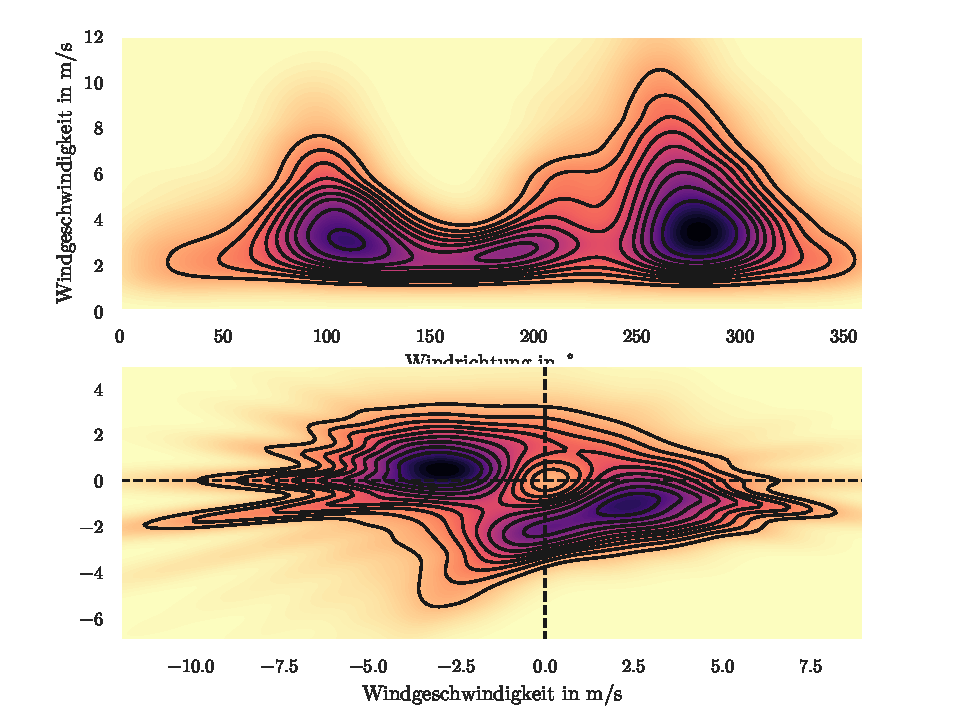
\includegraphics[scale = 1]{./images/pol2cart_visualize.pdf}
		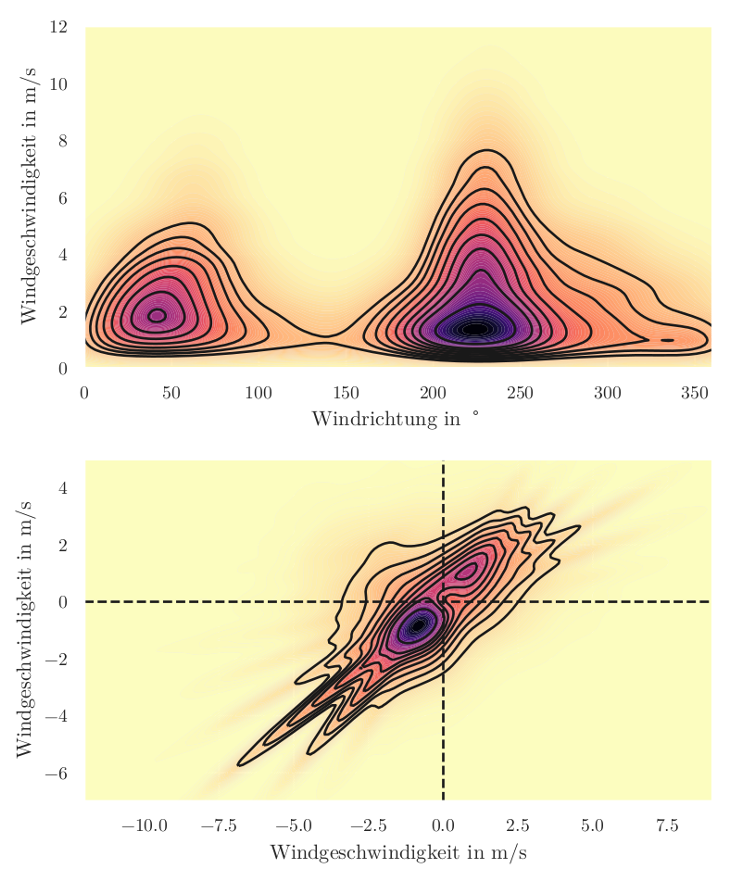
\includegraphics[scale = 1]{./images/pol2cart.png}
		\caption{Verteilung des Windes bei $(v,\varphi)$ bzw. $(v_x,v_y)$-Interpretation für die Messtation Günzburg im Zeitraum 01.2016 bis 03.2021}
		\label{fig:pol2cart2}
	\end{center}
\end{figure}
%%%%%BILD ENDE

\subsection{Normierung}

Es ist im Bereich des maschinellen Lernens üblich die Eingabedaten im Zuge der Datenaufbereitung zu normieren. Das ist insbesondere für Daten mit stark unterschiedlichen Wertebereichen wichtig. 

Eine negative Temperatur mag zwar für den Menschen sehr intuitiv sein, für das neuronale Netz enthält das Vorzeichen jedoch keine relevanten Informationen. Auch ist die Änderung von $1010 hPa$ auf $980 hPa$ für den Menschen klar ersichtlich, relativ ist sie jedoch nur sehr gering. 

Zudem kann es passieren, dass eine Größe mit extrem großem Wertebereich gegenüber einer mit sehr kleinem Wertebereich als wichtiger erscheint und so dominant wirkt.

Übliche Funktionen sind die $z$-Normierung (Normierung über Standardabweichung und Mittelwert) sowie die $minmax$-Normierung (Normierung über Minimum und Maximum). In dieser Arbeit wurde die letztere genutzt. Die ursprünglichen und angepassten Wertebereiche können der Tabelle \ref{tab:messgrößen} entnommen werden.

%%%%%TABELLE ANFANG
\begin{table}[ht]
	\centering
	\caption{Normalisierung der Eingabedaten}
	\begin{tabular}{|c|c|c|c|c|c|c|c|}
		\hline
		\rowcolor{color80}
		\textbf{$X$} & \textbf{$w_x$} & \textbf{$w_y$} & \textbf{$p$} & \textbf{$T$} & \textbf{$RH$} & \textbf{$cal_{day}$} & \textbf{$cal_{seas}$} \\ \hline
		Einheit $X$ & $m/s$ & $m/s$ & $hPa$ & $^\circ C$ & \% & $1$ & $1$ \\ \hline
		$min(X)$       & $-22.1$ & $-13.7$ & $975.2$ & $-19.1$ & $10$ & $0$ & $0$ \\ \hline
		$max(X)$       & $13.5$ & $9.7$ & $1047.3$ & $34.4$ & $100$ & $1$ & $1$ \\ \hline
		$min(norm(X))$ & $-1$ & $-1$ & $0$ & $0$ & $0$ & $-$ & $-$ \\ \hline
		$max(norm(X))$ & $1$ & $1$ & $1$ & $1$ & $1$ & $-$ & $-$ \\ \hline
	\end{tabular}
\label{tab:normalisierung}
\end{table}
%%%%%TABELLE ENDE

\section{Generierung der Trainingsbeispiele}
Nachdem die Rohdaten aufgearbeitet worden sind, gilt es nun tatsächliche Trainingsbeispiele (Samples) zu generieren. Dieser Prozess wird in Abbildung \ref{fig:sampling} dargestellt, wobei die Grafik als Fortsetzung von Abbildung \ref{fig:preprocessing} verstanden werden kann. Das Ziel des Samplings ist die Generierung eins Pools aus Trainingsbeispielen, womit das neuronale Netz angelernt werden kann.

Zunächst müssen die Größen der Moving-Windows (siehe Abb. \ref{fig:sampling}) festgelegt werden. Bei den Inputdaten gibt die Größe $n$ des Moving-Windows an, wieviele historische Zeitschritte für die Prognose genutzt werden (im Folgenden Prognosehistorie genannt). Das heißt, bei einer Prognose zum Zeitpunkt $t_0$ werden die Daten zu den Zeitpunkten $t_{n-1}, \dots, t_0$ als Inputdaten verwendet. Die Größe $m$ des Moving-Window auf den Labeldaten gibt den Prognosehorizont an. Das Ziel ist es also bei einer Prognose zum Zeitpunkt $t_0$ die Windgeschwindigkeiten und Windrichtungen zu den Zeitpunkten $t_1, \dots, t_m$ vorherzusagen. In dieser Arbeit wurde für $n=144$ und für $m=12$ gewählt, die Prognosehistorie beträgt also sechs Tage und der Prognosehorizont zwölf Stunden. Diese Werte wurden unter Berücksichtigung der Literaturrecherche gewählt.

Das Ergebnis der Datenaufbereitung, beschrieben im Kapitel \ref{section:Datenaufbereitung}, sind datenlückenfreie Fragmentpaare. Ein solches Fragmentpaar besteht aus einem Input- und einem Labeldatensatz. Darüber werden nun die im vorherigen Schritt definierten Moving-Windows \qm{geschoben}. Die Schrittweite wird dabei kleinstmöglich gewählt, so entstehen am meisten Samples. Das Sampling wird auf jedem Fragmentpaar angewandt.

%%%%%BILD ANFANG
\begin{figure}[tph]
	\begin{center}
		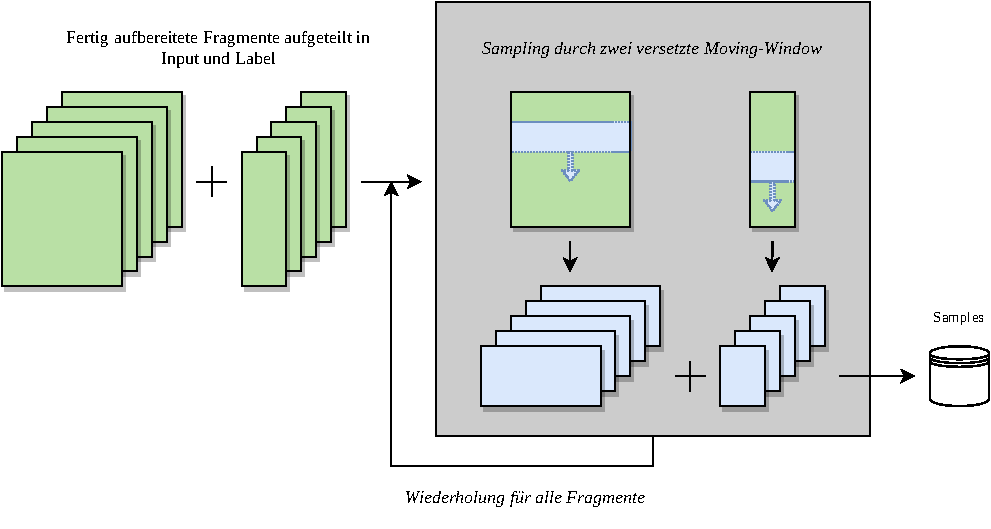
\includegraphics[]{./images/sampling.pdf}
		\caption{Generierung der Samples aus den aufbereiteten Fragmenten über zwei Moving-Windows.}
		\label{fig:sampling}
	\end{center}
\end{figure}
%%%%%BILD ENDE

Abschließend werden die Samples, wie in Anwendungen des maschinellen Lernens üblich \cite{2020_Shah_TrainValidationTest}, in drei Teile aufgeteilt. Diese haben die folgende Anwendung und Aufteilung:

\begin{itemize}
	\item \textit{Trainings-Satz, $65\%$}
	
	Mit diesen Samples wird das neuronale Netz tatsächlich trainiert. 

	\item \textit{Validierungs-Satz, $25\%$}
	
	Diese Samples werden beim Training zur Validierung genutzt. So kann Over- bzw. Underfitting erkannt werden.

	\item \textit{Test-Satz, $10\%$}
	
	Mit den restlichen Samples wird die Performance des neuronalen Netzes ermittelt. 

\end{itemize}

\chapter{Implementierung}

\section{Konfiguration des Modells}

Das Verhalten eines neuronalen Netzes ist von einer Vielzahl an Hyperparametern abhängig (u.a. Modellarchitektur, Lernraten und Lernverfahren, Initialisierung der Gewichte). Das Optimum aller Konfigurationen lässt sich im Allgemeinen nur annähern, wobei die Suche nach diesem einen großen zeitlichen und rechenintensiven Aufwand mit sich bringt.

Um den Aufwand in einem akzeptablen Maß zu halten, haben wir einige Parameter vorab festgelegt und andere iterativ bestimmt:

\begin{itemize}
	\item Vorab festgelegte Parameter
	\begin{itemize}
		\item Optimizer
		
		Als Optimizer wurde Adam gewählt. Er zeichnet sich durch eine hohe Konvergenzgeschwindigkeit und Robustheit aus und entspricht dem Stand der Technik. Die internen Abfallraten $\beta_1$ und $\beta_2$ liefern mit ihren Standardwerten im Allgemeinen gute Ergebnisse \cite{2017_Kingma_AdamMethodStochastic}, weshalb diese nicht verändert wurden. Die Lernrate wurde auf $0.001$ festgelegt.

		\item Lossfunktion
		
		Als Lossfunktion wurde MSE gewählt. Hier durch fallen besonders schlechte Prognosen stärker ins Gewicht.

	\end{itemize}

	\item Iterativ bestimmte Parameter
	\begin{itemize}
		\item Anzahl der Neuronen pro Schicht
		
		Die Anzahl der Neuronen einer Schicht haben großen Einfluss auf das Verhalten des Netzes, insbesondere in Hinblick auf Over- und Underfitting. Dabei wurden die Anzahl iterativ verändert und je nach Ausgang erhöht oder verringert. Auch wurde das Verhältnis der Neuronenanzahl zwischen zwei Schichten verändert. Im Folgenden wird eine Schicht mit $x$ bzw. $y$ Neuronen SCHICHT($x$) bzw. SCHICHT($y$) bezeichnet. $x$ und $y$ wurden dabei aus $[8,12,16,24,32,48,64,128]$ gewählt.

		\item Dropoutrate
		
		Eine Dropoutschicht hilft besonders bei rekrutenten neuronalen Netzen Overfitting sowie bekannte Probleme wie dem \qm{vanishing gradient} und \qm{exploding gradient} entgegenzuwirken. Die Dropoutrate definiert dabei den Prozentsatz an Neuronen, die zeitweise bei einem Lernschritt nicht berücksichtigt werden. Im Folgenden wird eine Dropoutschicht mit einer Rate $d$ als DROP($d$) bezeichnet. In dieser Arbeit wurde $d \in [0.1, 0.2, 0.3, 0.4]$ gewählt.
		\item Modellarchitektur
		
		Die Literaturrecherche hat gezeigt, dass die rekrutenten neuronalen Netze, speziell bei Verwendung von LSTM Zellen, sehr vielversprechende Ergebnisse liefern. Daher kommen in dieser Arbeit ebenso neuronale Netze mit LSTM Zellen zum Einsatz. Die Modellarchitektur hat großen Einfluss auf das Prognoseergebnis, weshalb mehrere Architekturen getestet wurden. $x$ und $y$ sind dabei die Anzahl der Neuronen und $d$ die Dropoutrate. Die Anzahl der Neuronen in der Eingabeschicht IN und Ausgabeschicht OUT wird durch den Datensatz definiert und wird hier nicht festgelegt:

		\begin{itemize}
			\item IN – LSTM($x$) – DROP($d$) – DENSE($y$) – DROP($d$) – OUT
			\item IN – LSTM($x$) – DROP($d$) – LSTM($y$) – DROP($d$) – OUT
			\item IN – LSTM($x$) – DROP($d$) – LSTM($y$) – OUT
			\item IN – DENSE($x$) – DROP($d$) – LSTM($y$) – OUT
			\item IN – LSTM($x$) – DROP($d$) – DENSE($y$) – OUT
			\item IN – LSTM($x$) – DROP($d$) – DENSE($x$) – DROP($d$) – DENSE($y$) – OUT

		\end{itemize}


		
	\end{itemize}
\end{itemize}


\section{Ergebnisse}\label{section:ergebnisse_training}
Insgesamt wurden 71 neuronale Netze mit jeweils unterschiedlichen Konfigurationen trainiert. Während des Trainings wurde das Modell zwischengespeichert, wenn sich die Prognosegüte nach einer Epoche verbessert hat. Das Training wurde nach 10 Epochen, in denen sich die Güte nicht verbessert hat, abgebrochen. Trainiert wurde stets mit dem Datensatz, bei dem der Wind in eine x- und y-Komponente umgewandelt worden ist. Die nachfolgende Tabelle fässt das Training und die Prognosegüte zusammen:

\begin{table}[ht]
	\centering
	\caption{Zusammenfassung der Konfigurationen der trainierten Netze.}
	\begin{tabular}{|C{2.5cm}|C{1.8cm}|C{2cm}|C{2cm}|C{2cm}|C{1.8cm}|C{1.8cm}|}
	\hline
	\rowcolor{color80}
	\textbf{Netzwerk Architektur} & \textbf{Anzahl trainierter Netze} & \textbf{Anzahl $x$ Neuronen} & \textbf{Anzahl $y$ Neuronen} & \textbf{Dropout-rate $d$} & \textbf{$MAE$ bestes Modell} & \textbf{$MSE$ bestes Modell} \\
	\hline
	IN – LSTM(x) – DROP(d) – DENSE(y) – DROP(d) – OUT & 9 & 8-32 & 8-96 & 0,3 & 0,8743 & 1,35 \\
	\hline
	IN – LSTM(x) – DROP(d) – LSTM(y) – DROP(d) – OUT & 9 & 16-64 & 16-64 & 0,3 & 0,8734 & 1,3448 \\
	\hline
	IN – LSTM(x) – DROP(d) – LSTM(y) – OUT & 10 & 16-64 & 8-32 & 0,2-0,3 & 0,8697 & 1,3378 \\
	\hline
	IN – DENSE(x) – DROP(d) – LSTM(y) – OUT & 15 & 26-64 & 16-32 & 0,2-0,4 & \textbf{0,8576} & \textbf{1,2807} \\
	\hline
	IN – LSTM(x) – DROP(d) – DENSE(y) – OUT & 19 & 16-32 & 16-32 & 0,1-0,3 & 0,8664 & 1,3212 \\
	\hline
	IN – LSTM(x) – DROP(d) – DENSE(x) – DROP(d) – DENSE(y) – OUT & 9 & 16-128 & 12-64 & 0,3 & 0,8643 & 1,3022\\
	\hline
	\end{tabular}
\end{table}

%%%%%%%%%%%%%%%%%%%%%%%%%%%%%%%%%%%%%%%%%%%%%%%%%%%%%%%%%%%%%%%%%%%%%%%
%                                                                     %
%                                                                     %
%                                                                     %
%                               KAPITEL                               %
%                                                                     %
%                                                                     %
%                                                                     %
%%%%%%%%%%%%%%%%%%%%%%%%%%%%%%%%%%%%%%%%%%%%%%%%%%%%%%%%%%%%%%%%%%%%%%%

\chapter{Diskussion und Ausblick}

In diesem Kapitel werden die erhaltenen Ergebnisse zunächst eingeordnet und kritisch betrachtet.
Im Anschluss werden Verbesserungsmöglichkeiten des Modells und neue Ansätze für die Fragestellungen dieser Arbeit aufgeführt, welche die erhaltenen Ergebnisse verbessern können, jedoch im Rahmen dieser Arbeit nicht ausgeführt werden konnten.

\section{Diskussion der Ergebnisse}\label{section:diskussion_ergebnisse}
Zunächst werden folgend die Fragen aufgeführt, welche im Rahmen dieser Arbeit beantwortet werden sollen.


\begin{itemize}
	\item Wie wirkt sich die in Kapitel \ref{section:Winddaten_vec} beschriebene Vektorisierung der Windgeschwindigkeit und Windrichtung auf die Prognose aus?
	\item Wie wirkt sich die Einbeziehung weiterer westlich gelegener Messstationen auf die Prognosegüte aus?
\end{itemize}

Um diese zu beantworten wurde das optimierte Modell aus Kapitel \ref{section:ergebnisse_training} mit folgenden drei Datensätzen trainiert:

\begin{itemize}
	\item Messdaten aller Messstationen, Windgeschwindigkeit und Windrichtung vektorisiert + kalendarische Daten
	\item Messdaten aller Messstationen, Windgeschwindigkeit und Windrichtung nicht vektorisiert + kalendarische Daten
	\item Messdaten nur von der Messstation Günzburg, Windgeschwindigkeit und Windrichtung vektorisiert + kalendarische Daten
\end{itemize}

Rückblickend muss an dieser Stelle auf zwei methodische Fehler hingewiesen werden. Zum einen fehlt hier ein vierter Datensatz, in dem die Winddaten nicht vektorisiert vorliegen und nur die Daten der Messtation Günzburg beinhaltet. So wäre der Vergleich untereinander aussagekräftiger. Der zweite methodische Fehler betrifft die Auswahl des besten Modells. Die optimale Konfiguration des neuronalen Netzes wurde mit dem ersten Datensatz ermittelt. Das bedeutet aber auch, dass die Konfiguration \textit{genau} auf diesen Datensatz \qm{maßgeschneidert} ist. Wir nutzen diese Konfiguration jedoch für alle drei Datensätze. Deutlich besser wäre es gewesen, für jeden Datensatz eine eigene optimale Konfiguration zu ermitteln. Durch diesen Fehler ist es möglich, dass die Performance des neuronalen Netzes mit Datensatz zwei und drei besser ist als im Folgenden beschrieben.

Diese methodischen Fehler müssen bei der Beurteilung der folgenden Analysen stets mit berücksichtigt werden.

\subsection{Klassische Performance Indikatoren}\label{section:klassische_perf_indi}
Für die Analyse der Performance eines neuronalen Netzes im Bereich regressiver Problemstellungen eigen sich die Fehlermaße MAE und MSE (wie auch die Literatur bestätigt) gut. Die Vorteile liegen beim MAE in der Liniarität und dadruch in der einfachen Verständlichkeit, wohingegen der MSE deutlich sensibler auf Ausreißer reagiert und so weitere interessante Informationen liefern kann.

In den Abbildungen \ref{fig:barplot_mae} und \ref{fig:barplot_mse} ist der MAE bzw. MSE für die drei Datensätze aufgetragen. Vergleicht man diese Grafiken, so lassen sich (zusätzlich zu den in Kapitel \ref{section:klassische_perf_indi} bereits diskutierten) folgende Erkenntnisse festhalten:

\begin{itemize}
	\item Werden die Fehlermaße für die Datensätze \qm{Wind vektorisiert, alle Messstationen} und \qm{Wind nicht vektorisiert, alle Messstationen} miteinander verglichen, so fällt auf, dass die Windgeschwindigkeit deutlich besser prognostiziert werden kann, wenn die Winddaten vektorisiert vorliegen. 
	
	Für die Prognose der Windrichtung kann kein intuitives Ergebnis aus den Grafiken entnommen werden. Zwar ist der MAE der vektorisierten Winddaten geringfügig kleiner als für die nicht vektorisierten, der MSE für die vektorisierten Winddaten hingegen ist größer. Hierbei muss jedoch beachtet werden, dass das neuronale Netz im Falle der vektorisierten Winddaten Informationen über die zirkulären Eigenschaften besitzt. So ist beispielsweise eine Prognose von $10^\circ$ anstatt $350^\circ$ mit einem Delta von $20^\circ$ relativ gut, die Fehlermaße interpretieren dies jedoch als ein Delta von $340^\circ$. Das deutlich höhere Fehlermaß MSE für den Datensatz \qm{Wind vektorisiert, alle Messstationen} gegenüber dem Datensatz \qm{Wind nicht vektorisiert, alle Messstationen} kann sich also über die hohe Sensitivität für Ausreißer beim MSE erklären lassen.

	Idealer Weise wäre also ein Fehlermaß, welches die Zirkularität und somit nur die tatsächliche Differenz  berücksichtigt. Dies wäre über den Sinus und Kosinus möglich. Da dieses Fehlermaß nicht implementiert wurde, muss für die Beurteilung der Prognosegüte der Windrichtung auf den etwas robusteren MAE zurückgegriffen werden.

	\item Bei dem Vergleich beider Fehlermaße für die Datensätze \qm{Wind vektorisiert, alle Messstationen} und \qm{Wind vektorisiert, nur Messstation Günzburg} fällt auf, dass die Windgeschwindigkeit besser prognostiziert werden kann, wenn die Daten aller Messstationen berücksichtigt werden. 
	
	Für die Prognosegüte der Windrichtung kann keine Verbesserung festgestellt werden.\\
	(Einerseits $MAE_{Alle} < MAE_{Eine}$, andererseits $MSE_{Alle} > MSE_{Eine}$)
\end{itemize}

%%%%%BILD ANFANG
\begin{figure}[tph]
	\begin{center}
		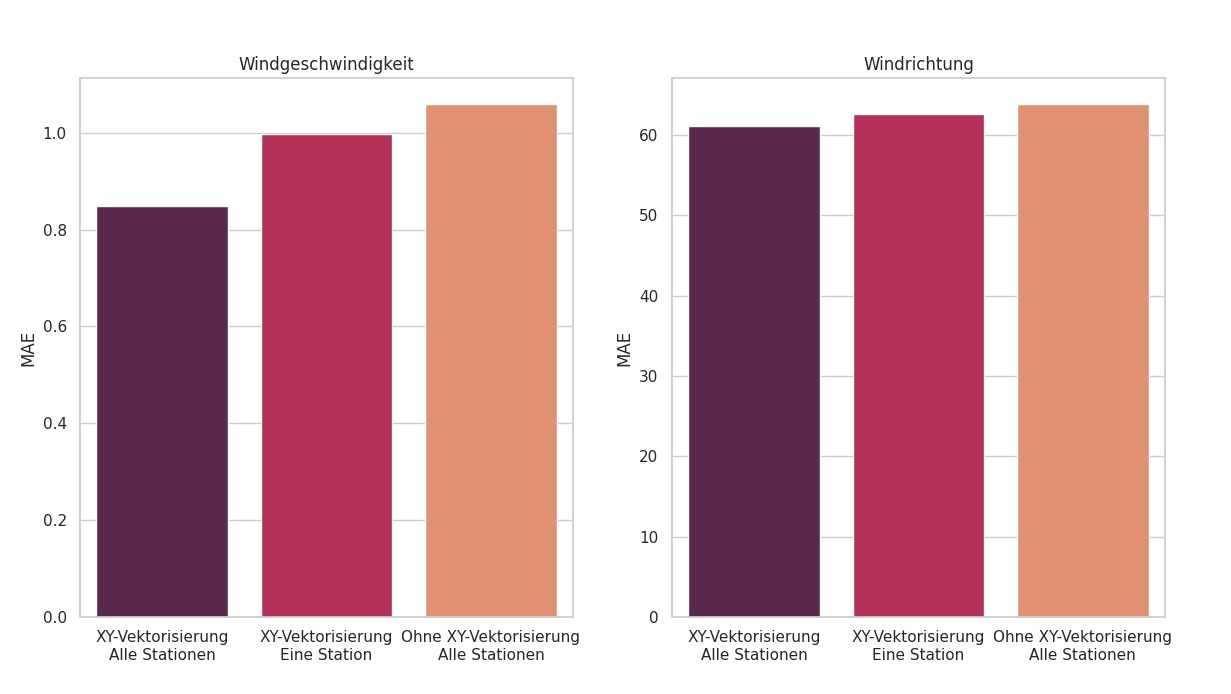
\includegraphics[width=\linewidth]{./images/barplot_mae-cropped.jpg}
		\caption{Mittlerer absoluter Fehler für die drei Datensätze im Vergleich}
		\label{fig:barplot_mae}
	\end{center}
\end{figure}
%%%%%BILD ENDE

%%%%%BILD ANFANG
\begin{figure}[tph]
	\begin{center}
		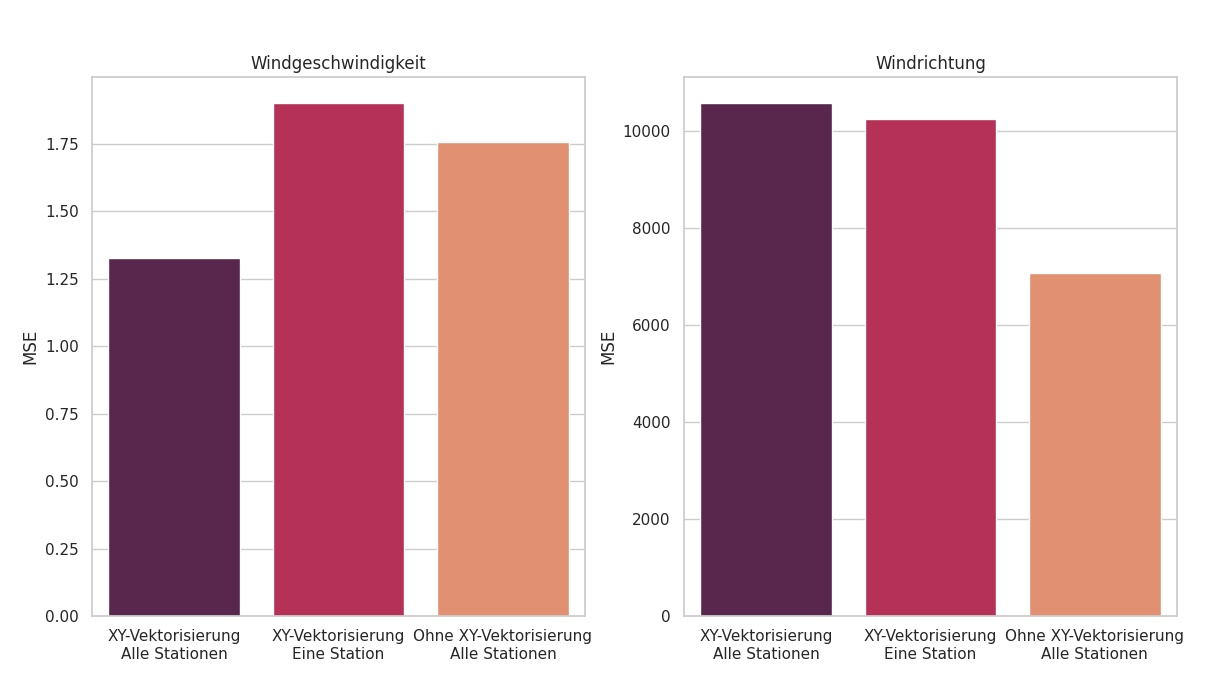
\includegraphics[width=\linewidth]{./images/barplot_mse-cropped.jpg}
		\caption{Mittlerer quadratischer Fehler für die drei Datensätze im Vergleich}
		\label{fig:barplot_mse}
	\end{center}
\end{figure}
%%%%%BILD ENDE

\subsection{Detaillierte Prognosegüte}
Um ein generelles Verständnis zu erlangen, wie gut die Prognose eines neuronalen Netzes ist, eigenen sich die klassischen Performance Indikatoren sehr gut. Auch sind sie hilfreich für Vergleiche mit anderen Prognosemodellen. 
Für ein detailliertes Verständnis reichen sie jedoch nicht aus. 

In dieser Arbeit wurde ein Prognosehorizont von zwölf Stunden gewählt. Trägt man die Prognosegüte über dem Prognosehorizont auf, erhält man einen detaillierteren Einblick über die Vorhersage. Abbildung \ref{fig:güte_über_zeit_xy_all},  \ref{fig:güte_über_zeit_xy_single} und  \ref{fig:güte_über_zeit_sd_all} zeigen dies für die drei Datensätze.

Vergleicht man die drei Grafiken, so lassen sich folgende Schlüsse ziehen:

\begin{itemize}
	\item Je ferner die Vorhersage in der Zukunft liegt, desto größer wird Fehler der Prognose sowohl für die Windgeschwindigkeit als auch für die Windrichtung. Lediglich der Fehler der Windgeschwindigkeit für den Datensatz \qm{Wind nicht vektorisiert, alle Messstationen} ist im Vergleich auch für unmittelbare Prognosen hoch.
	\item Sehr große Ausreißer ($MAE > 6$) für die Prognose der Windgeschwindigkeit treten fast ausschließlich für den Datensatz \qm{Wind vektorisiert, nur Messstation Günzburg} auf. Es scheint also als wäre die Prognose nicht nur besser, sondern auch robuster wenn alle Messstationen genutzt werden.
	\item In 75\% der Fälle (Quantil 3, Oberkante Boxplot) ist die Abweichung zwischen der prognostizierten und wahren Windgeschwindigkeit kleiner als $1.8 m/s$. In 50\% der Fälle (Median, Strich in Boxplot) ist der Fehler bereits unter $1 m/s$.
	\item Nur für $t_1$ und $t_2$ und nur bei vektorisierten Winddaten ist der Fehler in 75\% aller Fälle für die prognostizierte Windgeschwindigkeit kleiner als $45^\circ$ (\qm{akzeptabler Fehler}, entspricht dem Unterschied zwischen Wind aus Süd und Wind aus Südwest)
\end{itemize}

%%%%%BILD ANFANG
\begin{figure}[tph]
	\begin{center}
		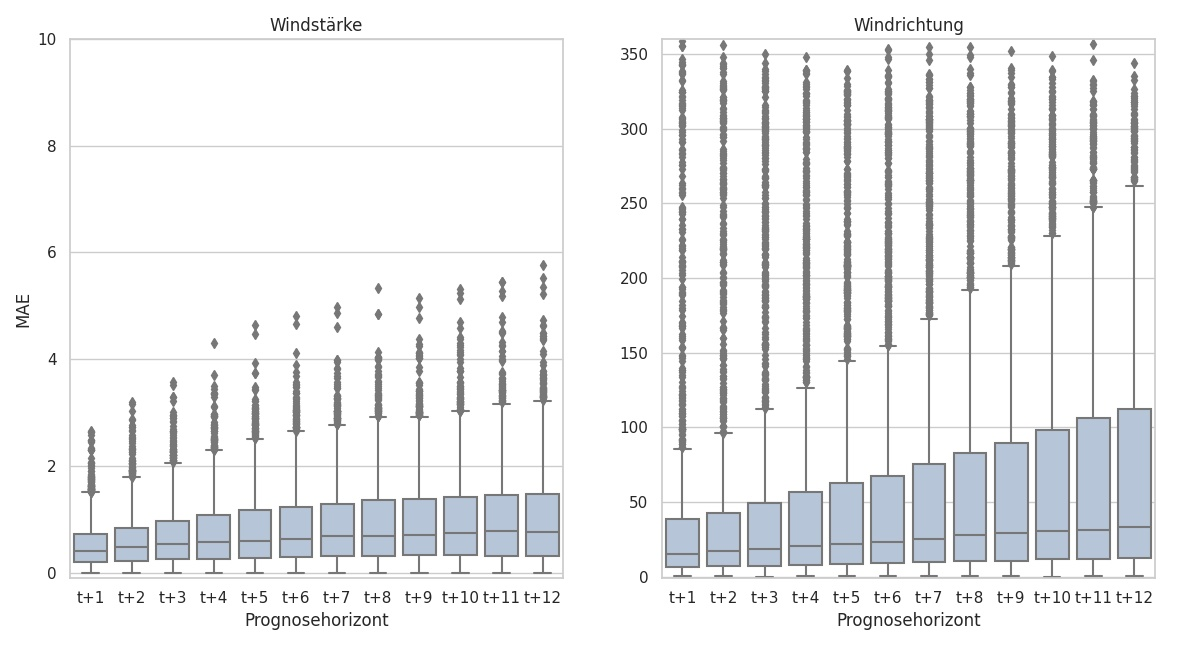
\includegraphics[width=\linewidth]{./images/Güte über Prognosehorizont sd via xy-cropped.jpg}
		\caption{Prognosegüte über Prognosehorizont für den Datensatz \qm{Wind vektorisiert, alle Messstationen}}
		\label{fig:güte_über_zeit_xy_all}
	\end{center}
\end{figure}
%%%%%BILD ENDE

%%%%%BILD ANFANG
\begin{figure}[tph]
	\begin{center}
		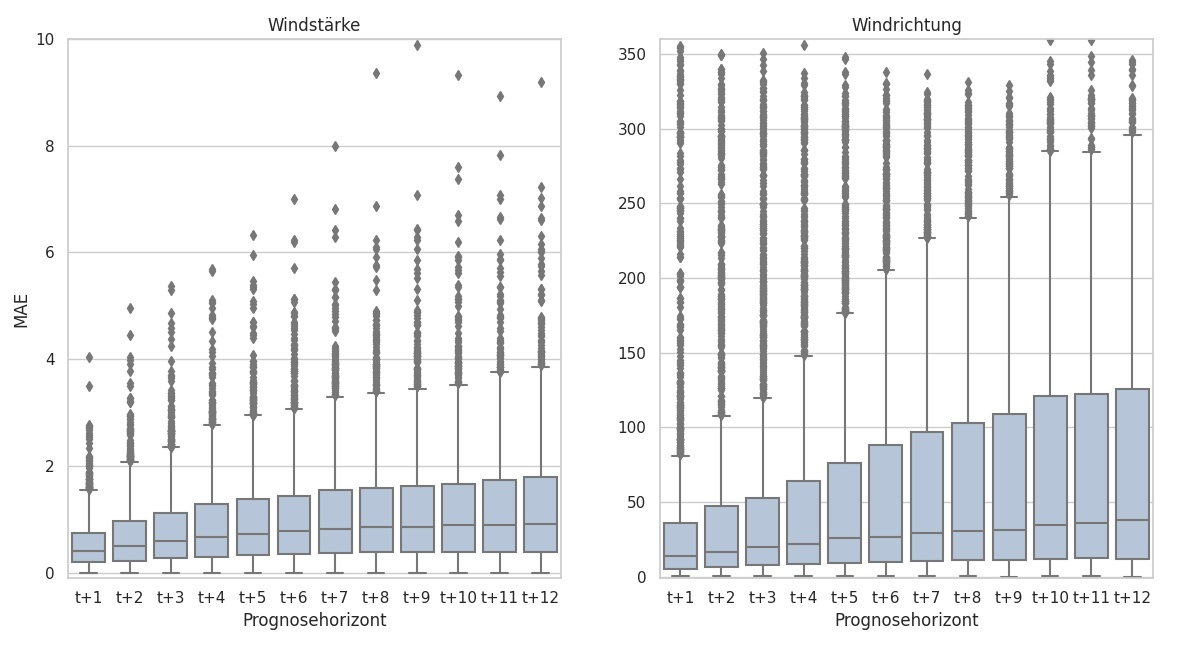
\includegraphics[width=\linewidth]{./images/Güte über Prognosehorizont sd single-cropped.jpg}
		\caption{Prognosegüte über Prognosehorizont für den Datensatz \qm{Wind vektorisiert, nur Messstation Günzburg}}
		\label{fig:güte_über_zeit_xy_single}
	\end{center}
\end{figure}
%%%%%BILD ENDE

%%%%%BILD ANFANG
\begin{figure}[tph]
	\begin{center}
		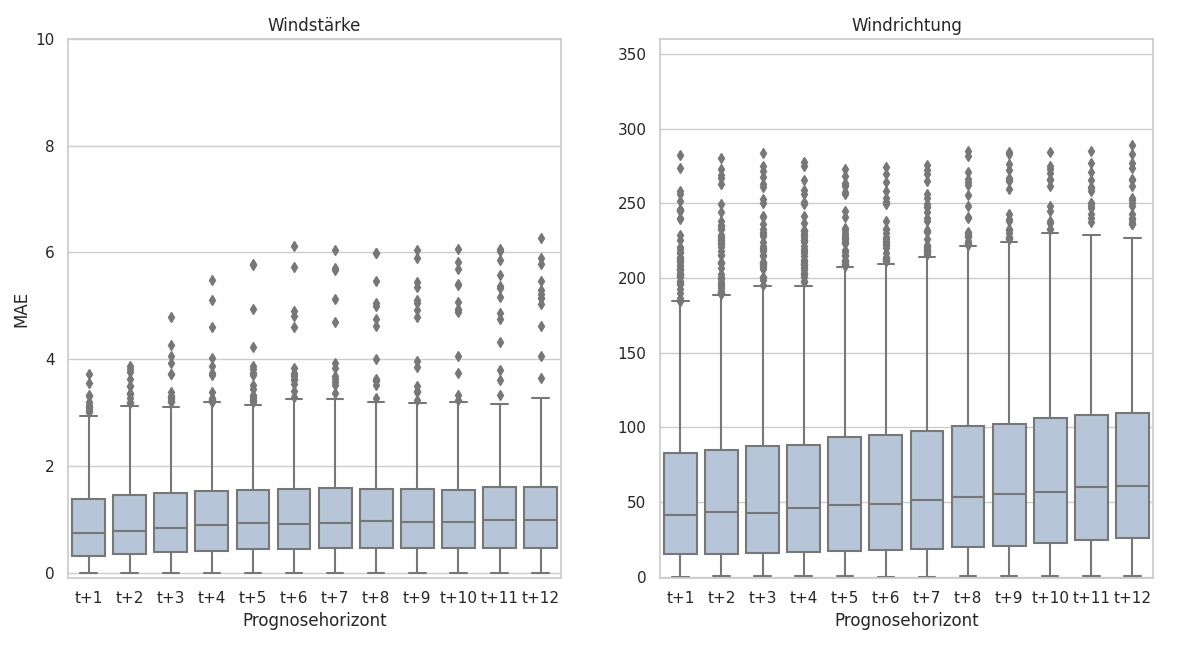
\includegraphics[width=\linewidth]{./images/Güte über Prognosehorizont sd direkt-cropped.jpg}
		\caption{Prognosegüte über Prognosehorizont für den Datensatz \qm{Wind nicht vektorisiert, alle Messstationen}}
		\label{fig:güte_über_zeit_sd_all}
	\end{center}
\end{figure}
%%%%%BILD ENDE

\section{Diskussion der kalendarischen Features}

Bei der Präsentation dieser Arbeit wurde die Sinnhaftigkeit der kalendarischen Daten als Features hinterfragt, da Saisonalitäten in den Winddaten und in der Temperatur selbst zu erkennen sind. Daher wurde aus dem Datensatz \qm{Wind vektorisiert, alle Messstationen} ein vierter Datensatz erzeugt, in dem die Features \textit{kalendarischer Tageswert} $cal_{day}$ und \textit{kalendarischer Saisonalwert} $cal_{seas}$ auf null gesetzt wurden. Zu jedem Zeitpunkt gilt also $cal_{day} = cal_{seas} = 0$. Das neuronale Netz kann hieraus keine Information ziehen und die Gewichte zu den jeweiligen Neuronen werden im Trainingsprozess \qm{genullt}.

Vergleicht man nun die Prognosegüte für den Datensatz \qm{Wind vektorisiert, alle Messstationen} mit dem eben beschriebenen, so stellt man fest, dass die kalendarischen Daten durchaus wertvolle Informationen beinhalten. Der MAE verschlechtert sich durch die fehlenden kalendarischen Informationen von $0.8576$ auf $0.8911$, der MSE von $1.2807$ auf $1.3862$. Dies entspricht einer relativen Verschlechterung von $3.9\%$ bzw. $8.2\%$.


\section{Weiterentwicklung des Modells}

Im Laufe der Arbeit kamen einige Verbesserungmöglichkeiten und Ideen auf. Einige sind Verbesserungen und Veränderungen innerhalb dieser Seminararbeit. 
Andere Ideen schlagen vollkommen neuartige Ansätze vor. Im Folgenden beschriebene Ideen können in Folgearbeiten näher betrachtet werden.

\subsection{Veränderungsvorschläge}

Kapitel \ref{section:diskussion_ergebnisse} umfasst eine genauere Beschreibung des methodischen Fehlers, welcher einen direkten Vergleich zwischen der unterschiedlichen Darstellung des Windes als Vektor verhindert. 
Zum einen wäre es sinnvoll einen vierten Datensatz hinzuzufügen, welcher die Daten der Station Günzburg beinhaltet und die Winddaten in nicht vektorisierter Form vorliegen hat. 
Der Vergleich der Ergebnisse kann dadurch deutlich mehr an Aussagekraft gewinnen. 
Darüber hinaus wurden die optimalen Modellparameter anhand des ersten Datensatzes gefunden. 
Es sollten noch weitere optimale Modellparameter für die anderen Datensätze verwendet werden um herauszufinden, ob sich die Prognosegüte mithilfe dieser neuen Konfigurationen verbessern kann. 
\newline
Dem vorigen Gedanken folgend könnte eine separate Optimierung zweier Modelle, eines um Windrichtung und eines um Windgeschwindigkeit vorherzusagen, die jeweils besten Prognosen ergeben. Hiermit erübrigen sich sogar die Überlegungen zu den unterschiedlichen Darstellungsweisen des Windes als Vektor.  
\newline
Bereits in Kapitel \ref{section:realeMessdaten} wurde darauf hingewiesen, dass einige der berücksichtigten Messstationen sehr wechselhafte Winddaten besitzen. Die Verwendung von Messdaten eines oder mehrerer Standorte in Küstenlage könnten einen guten Vergleich herstellen. 
Die Windlage an Küsten dürfte eindeutiger sein, als die im süddeutschen Raum. Bessere Ergebnisse bei einem gleichen verwendeten Modell würden bedeuten, dass das vorgestellte Modell nicht gut mit volatilen Winddaten umgehen kann und das Modell dementsprechend angepasst werden sollte.
\newline
In dieser Arbeit wurden Messdaten des Deutschen Wetterdienstes verwendet, welche häufig Datenlücken enthielten. Es könnten darüber hinaus Satellitendaten verwendet werden, auf die während auftretender Fehlstellen zurückgegriffen werden kann. 
Diese Vorgehensweise kann zu einer größeren Datenvielfalt und somit möglicherweise zu besseren Ergebnissen führen.
\newline
\citeauthor{2019_Chen_MultifactorSpatiotemporalCorrelation} \cite{2019_Chen_MultifactorSpatiotemporalCorrelation} konnten mittels einer Multifactor Spatiotemporal Correlation 3D-Matrix in ihren Eingabedaten zur selben Zeit mehrere Korrelationen zwischen Standorten und meteorologischen Faktoren in zeitlicher und räumlicher Dimension berücksichtigen. 
Da das in dieser Arbeit vorgestellte Modell ebenfalls die Daten mehrerer Standorte mit einbezieht, könnte die Anwendung dieser Methode in der Datenaufbereitung zu verbesserten Ergebnissen führen. 
\newline
In dieser Arbeit wurden die Ergebnisse mit üblichen Fehlermaßen bewertet. Ideen innerhalb dieses Modells, wie die andere Darstellung des Windvektors oder die Verwendung mehrerer Standorte in den Inputdaten, wurden dann mit dem Standardmodell verglichen. 
Jedoch ist dadurch unklar, wie gut das Modell im Gegensatz zu anderen üblichen Modellen abschneidet. Ein Vergleich mit einem häufig verwendeten Modell, wie dem SARIMA Modell, könnten aufschlussreiche Informationen liefern. 
Schneiden nämlich beide Modelle weniger gut ab, so sollten Prozesse in der Datenaufbereitung verändert werden oder neue Daten von anderen Standorten verwendet werden. Ein Vergleichsmodell sollte in einer weiterführenden Arbeit verwirklicht werden, um die hier enstandenen Ergebnisse einordnen zu können und mögliche Verbesserungsmöglichkeiten aufzudecken.

\subsection{Neue Ansätze}

Das Modell, welches \citeauthor{2019_Chen_MultifactorSpatiotemporalCorrelation} in ihrem Paper im Jahr 2019 vorstellten \cite{2019_Chen_MultifactorSpatiotemporalCorrelation} ist aufgrund der Verwendung von Messdaten mehrerer Standorte dem hier entwickelten Modell sehr ähnlich. 
\citeauthor{2019_Chen_MultifactorSpatiotemporalCorrelation} verwendeten kein RNN, sondern ein CNN mit LSTM Zellen. Ein CNN könnte für den Umgang mit mehreren Input-Standorten geeigneter sein als ein RNN.
\newline
Eine weiterführende Idee davon wäre ein Ensemble-Modell, wie beispielsweise das Modell der Forschungsgruppe \citeauthor{2017_Zhang_HybridMethodShortTerm} \cite{2017_Zhang_HybridMethodShortTerm}, zu entwickeln. Hierbei werden mehrere Prognoseansätze, welche jeweils gute Prognosen bei unterschiedlicher Datenbasis liefern können, kombiniert. 
Hierbei können jeweils die Stärken der Ansätze ausgenutzt werden und due Schwächen anderer verringert werden. Einen solchen Ansatz zu entwickeln wäre für eine zukünftige Arbeit äußerst interessant.
%%%%%%%%%%%%%%%%%%%%%%%%%%%%%%%%%%%%%%%%%%%%%%%%%%%%%%%%%%%%%%%%%%%%%%%
%                                                                     %
%                                                                     %
%                                                                     %
%                               KAPITEL                               %
%                                                                     %
%                                                                     %
%                                                                     %
%%%%%%%%%%%%%%%%%%%%%%%%%%%%%%%%%%%%%%%%%%%%%%%%%%%%%%%%%%%%%%%%%%%%%%%
% \chapter{Test und Wissen}

% \section{Tabelle}
% %%%%%TABELLE ANFANG
% \begin{table}[ht]
% 	\centering
% 	\caption{Das hier ist eine Testtabelle, man beachte die gezwungene Breite in der rechten Spalte. Lässt sich einfach durch den Befehl C\{5cm\} erzeugen.}
% 	\begin{tabular}{|l|C{5cm}|}
% 		\hline
%         \rowcolor{color80}
% 		\textbf{Erste Zelle}&\textbf{Ein Header}\\
% 		\hline
% 		Moin: & Zusammen\\\hline
% 		leer:&\\\hline
% 		Moin: & Zusammen\\\hline
% 		leer:&\\\hline
% 	\end{tabular}
% \label{tab:testtabelle}
% \end{table}
% %%%%%TABELLE ENDE

% %%%%%LANGTABELLE ANFANG
% \begin{longtable}{|L{3.6cm}|L{6cm}|L{6cm}|}
% 	\caption{Finale Merkmale}\label{tab:longtable}\\
%     % Definition des Tabellenkopfes auf der ersten Seite
% 	\hline
%     \rowcolor{color80}
% 	\textbf{Abkürzung}&\textbf{Englisch}&\textbf{Deutsch}\\
% 	\hline
% 	\endfirsthead % Erster Kopf zu Ende
% 	% Definition des Tabellenkopfes auf den folgenden Seiten
% 	\hline
% 	\rowcolor{color80}
% 	\textbf{Abkürzung}&\textbf{Englisch}&\textbf{Deutsch}\\
% 	\hline
% 	\endhead % Zweiter Kopf ist zu Ende
%     \hline
%     \endfoot
%     \hline
%     \endlastfoot
% 	% Ab hier kommt der Inhalt der Tabelle
% 	$test_{\mathrm{abk}}$&ein sehr sehr sehr langertextmit langen wörternein sehr sehr sehr langertextmit langen wörternein sehr sehr sehr langertextmit langen wörternein sehr sehr sehr langertextmit langen wörternein sehr sehr sehr langertextmit langen wörtern&Einzeilig\\
% 	Z&5&as\\\hline
% 	A&1&91\\\hline
% 	B&2&97\\\hline
% 	Z&5&as\\\hline
% 	A&1&91\\\hline
% 	B&2&97\\\hline
% 	A&1&91\\\hline
% 	B&2&97\\\hline
% 	Z&5&as\\\hline
% 	A&1&91\\\hline
% 	B&2&97\\\hline
%     Z&5&as\\\hline
% 	A&1&91\\\hline
% 	B&2&97\\\hline
% 	Z&5&as\\\hline
% 	A&1&91\\\hline
% 	B&2&97\\\hline
%     Z&5&as\\\hline
% 	A&1&91\\\hline
% 	B&2&97\\\hline
% 	Z&5&as\\\hline
% 	A&1&91\\\hline
% 	B&2&97\\\hline
%     Z&5&as\\\hline
% 	A&1&91\\\hline
% 	B&2&97\\\hline
% 	Z&5&as\\\hline
% 	A&1&91\\\hline
% 	B&2&97\\\hline
%     Z&5&as\\\hline
% 	A&1&91\\\hline
% 	B&2&97\\\hline
% 	Z&5&as\\\hline
% 	A&1&91\\\hline
% 	B&2&97\\\hline
%     Z&5&as\\\hline
% 	A&1&91\\\hline
% 	B&2&97\\\hline
% 	Z&5&as\\\hline
% 	A&1&91\\\hline
% 	B&2&97\\\hline
% 	Z&5&as\\\hline
% 	A&1&91\\\hline
% 	B&2&97\\\hline
% 	Z&5&as\\\hline
% 	A&1&91\\\hline
% 	B&2&97\\\hline
% 	Z&5&KEINE hline AM SCHLUSS!!!\\
% \end{longtable}
% %%%%%LANGTABELLE ENDE

% \section{Bild}

% %%%%%BILD ANFANG
% \begin{figure}[tph]
% 	\begin{center}
% 		
\includegraphics[scale = 1]{./images/0_testbild.png}
% 		\caption{TEST Hier ist ein wunderschönes Testbild zu erkennen, und das hier ist ein wunderschönes Testbild zu erkennen, und das hier ist ein wunderschönes Testbild zu erkennen, und das hier ist ein wunderschönes Testbild zu erkennen, und das hier ist ein wunderschönes Testbild zu erkennen, und das hier ist ein wunderschönes Testbild zu erkennen, und das hier ist ein}
% 		\label{fig:testbild}
% 	\end{center}
% \end{figure}
% %%%%%BILD ENDE

% %%%%%DOPPELBILD ANFANG
% \begin{figure}
% 	\centering
% 	\begin{minipage}[b]{.4\linewidth} % [b] => Ausrichtung an \caption
% 		
\includegraphics[width=\linewidth]{./images/0_testbild.png}
% 		\caption{Beschreibung und so}
% 		\label{fig:testbild_klein_links}
% 	\end{minipage}
% 	\hspace{.1\linewidth}% Abstand zwischen Bilder
% 	\begin{minipage}[b]{.4\linewidth} % [b] => Ausrichtung an \caption
% 		
\includegraphics[width=\linewidth]{./images/0_testbild.png}
% 		\caption{Zweite Beschreibung}
% 		\label{fig:testbild_klein_rechts}
% 	\end{minipage}
% \caption*{Hier steht eine etwas längere Bildunterschrift, die dieses Doppelbild beschreibt. Zu sehen sind weder Land noch Wasser, das macht bei Testbildern aber nix.}
% \end{figure}
% %%%%%DOPPELBILD ENDE

% \section{Formeln}

% Aufpassen, hier kommt jetzt eine einfache Testformel hin:

% \begin{equation}
% \label{eq:1}
% x=10
% \end{equation}

% Diese Formel \autoref{eq:1} kann auch referenziert werden.

% \begin{equation}
% x=Ma_{\mathrm{blabla}} \cdot y
% \end{equation}

% \section{Zitate}

% Um Bib zu kompilieren, einmal F8 drücken.

% Bild \autoref{fig:testbild} referenzieren.
% %Auch ein Autorname \citeauthor{ernstGrundkursInformatikGrundlagen2015} oder ein Jahr geht \citeyear{ernstGrundkursInformatikGrundlagen2015}

%%%%%%%%%%%%%%%%%%%%%%%%%%%%%%%%%%%%%%%%%%%%%%%%%%%%%%%%%%%%%%%%%%%%%%%
%                                                                     %
%                                                                     %
%                                                                     %
%                               KAPITEL                               %
%                                                                     %
%                                                                     %
%                                                                     %
%%%%%%%%%%%%%%%%%%%%%%%%%%%%%%%%%%%%%%%%%%%%%%%%%%%%%%%%%%%%%%%%%%%%%%%
\printbibliography[title=Literaturverzeichnis]
\end{document}